\documentclass[conference]{IEEEtran}
\IEEEoverridecommandlockouts
% The preceding line is only needed to identify funding in the first footnote. If that is unneeded, please comment it out.
\usepackage{cite}
\usepackage{amsmath,amssymb,amsfonts}
\usepackage{algorithmic}
\usepackage{graphicx}
\usepackage{textcomp}
\usepackage{xcolor}

\def\BibTeX{{\rm B\kern-.05em{\sc i\kern-.025em b}\kern-.08em
    T\kern-.1667em\lower.7ex\hbox{E}\kern-.125emX}}
\begin{document}

\title{Estudo Experimental de Associações de Resistores e Efeito Joule\\
    % {\footnotesize Relatório de Laboratório}
}
\author{\IEEEauthorblockN{1\textsuperscript{st} Arthur Cadore Matuella Barcella}
    \IEEEauthorblockA{\textit{Departamento de Telecomunicações} \\
        \textit{Instituto Federal de Santa Catarina}\\
        São José, Brasil \\
        arthur.cmb@aluno.ifsc.edu.br}
    \and
    \IEEEauthorblockN{2\textsuperscript{nd} Faber Bernardo Junior}
    \IEEEauthorblockA{\textit{Departamento de Telecomunicações} \\
        \textit{Instituto Federal de Santa Catarina}\\
        São José, Brasil \\
        faber.b@aluno.ifsc.edu.br}
    \and
    \IEEEauthorblockN{3\textsuperscript{rd} Gabriel Luiz Espindola Pedro}
    \IEEEauthorblockA{\textit{Departamento de Telecomunicações} \\
        \textit{Instituto Federal de Santa Catarina}\\
        São José, Brasil \\
        gabriel.ep@aluno.ifsc.edu.br}
}



\maketitle

\begin{abstract}
    Este trabalho apresenta uma análise experimental das associações de resistores em configurações série, paralelo e mista, utilizando componentes comerciais com valores nominais de \(1\,k\Omega\) e \(1\,M\Omega\). Foram realizadas medições de resistência, tensão e corrente, acompanhadas de análise estatística para avaliação das tolerâncias e incertezas associadas aos componentes. Além disso, investigou-se o efeito Joule por meio do aquecimento de uma amostra de água utilizando um resistor submerso, com modelagem matemática que incorpora a dissipação térmica e a transferência de calor para o ambiente. Os resultados evidenciam a importância do rigor experimental e da consideração das variabilidades dos componentes para a obtenção de resultados confiáveis, assim como a relevância do entendimento dos fenômenos térmicos em sistemas elétricos para o dimensionamento seguro e eficiente de dispositivos dissipadores de energia. Este estudo contribui para o aprofundamento dos conceitos teóricos e práticos fundamentais para a formação em engenharia elétrica e eletrônica.
\end{abstract}

\begin{IEEEkeywords}
    Associação de resistores, resistência elétrica, tolerância de componentes, análise estatística, efeito Joule.
\end{IEEEkeywords}


\section{Introdução}

% Este experimento tem como objetivo analisar o comportamento de associações de resistores em série e em paralelo, utilizando cinco resistores de $1 k\Omega$ e cinco de $1 M\Omega$. As medições serão realizadas em corrente contínua (CC), com o uso de multímetro e osciloscópio para observar as respostas dos circuitos.

% A compreensão de como a disposição dos resistores influencia a resistência total de um circuito é essencial na eletrônica. Além disso, este experimento proporciona experiência prática com instrumentos de medição e desenvolve habilidades em análise experimental.

A resistência elétrica é uma das grandezas fundamentais na eletricidade e na eletrônica, representando a oposição que um material oferece à passagem da corrente elétrica \cite{hayt2019analise}. Os resistores, componentes passivos projetados especificamente para introduzir resistência nos circuitos, são amplamente utilizados em sistemas eletrônicos e elétricos para controle de corrente, divisão de tensão e proteção de componentes sensíveis. O comportamento desses dispositivos, quando combinados em diferentes configurações, pode modificar significativamente as propriedades globais de um circuito \cite{boylestad2014dispositivos}.

Duas das principais formas de associação de resistores são as ligações em série e em paralelo. Na associação em série, os resistores são conectados de forma que a corrente que passa por todos é a mesma, e a resistência equivalente é a soma direta dos valores individuais \cite{hayt2019analise}. Já na associação em paralelo, todos os resistores compartilham os mesmos pontos de entrada e saída de tensão, mas a corrente se divide entre os caminhos disponíveis; nesse caso, a resistência total é calculada pelo inverso da soma dos inversos das resistências individuais \cite{hayt2019analise}. Compreender essas relações é essencial para o projeto e a análise de circuitos eletrônicos, desde os mais simples até os sistemas complexos utilizados em dispositivos modernos.

O entendimento teórico dessas associações está fundamentado na Lei de Ohm e nas Leis de Kirchhoff \cite{halliday}. A Lei de Ohm estabelece a relação linear entre a tensão, a corrente e a resistência, enquanto as Leis de Kirchhoff permitem analisar a conservação de corrente em nós (Lei das Correntes) e a conservação de energia em malhas (Lei das Tensões) \cite{halliday}. A aplicação dessas leis no contexto de circuitos com múltiplos resistores fornece uma base sólida para prever o comportamento elétrico de sistemas reais.

Neste experimento, propõe-se a análise de circuitos contendo resistores de $1,k\Omega$ e $1,M\Omega$, dispostos em diferentes combinações de série e paralelo. As medições serão realizadas em corrente contínua (CC), utilizando instrumentos como multímetros e osciloscópios, com o objetivo de verificar empiricamente os valores de tensão, corrente e resistência nos circuitos montados. Além da validação experimental dos conceitos teóricos, a atividade visa desenvolver competências práticas importantes, como a manipulação de componentes eletrônicos, a montagem de circuitos e o uso adequado de instrumentos de medição.

A realização desse tipo de experimento em ambiente laboratorial é essencial na formação de estudantes de engenharia e áreas afins, pois promove uma conexão direta entre teoria e prática. Ao observar na prática os efeitos da associação de resistores, os estudantes consolidam seus conhecimentos e desenvolvem uma intuição mais apurada sobre o funcionamento de circuitos elétricos, o que é indispensável para o desempenho em projetos futuros.

Este trabalho se organiza da seguinte forma % TODO: ESCREVER QUANDO TIVER PRONTO

\section{Revisão de literatura}

% As associações de resistores são fundamentais em circuitos elétricos.
% Em associação série, a resistência equivalente é dada pela soma dos valores individuais.
% Já em associação paralelo, a resistência equivalente é obtida pela soma dos inversos das resistências individuais \cite{hayt2019analise}.

% Em corrente alternada (CA), além da resistência,
% fatores como capacitâncias e indutâncias parasitas podem influenciar o comportamento do circuito, especialmente em altas frequências \cite{halliday}.
% O multímetro é utilizado para medir resistência, tensão e corrente em CC, enquanto o osciloscópio permite visualizar formas de onda e analisar a resposta dinâmica dos circuitos \cite{hayt2019analise}.

% Esta seção revisa os conceitos teóricos fundamentais para a análise experimental, reforçando a importância de compreender as associações resistivas e as limitações práticas dos instrumentos de medição.

As associações de resistores constituem a base da análise de circuitos elétricos e são amplamente abordadas em disciplinas introdutórias de eletricidade e eletrônica. Quando conectados em série, os resistores compartilham a mesma corrente elétrica, e a resistência equivalente do circuito é determinada pela soma direta dos valores individuais: $R_\text{eq} = R_1 + R_2 + \dots + R_n$. Por outro lado, na associação em paralelo, a tensão aplicada é a mesma em todos os resistores, e a resistência equivalente é dada pelo inverso da soma dos inversos das resistências: $1/R_\text{eq} = 1/R_1 + 1/R_2 + \dots + 1/R_n$ \cite{hayt2019analise}. Compreender essas configurações é essencial para o projeto e o diagnóstico de sistemas elétricos.

Em circuitos alimentados por corrente alternada (CA), a análise se torna mais complexa devido à presença de reatâncias associadas a componentes capacitivos e indutivos. Mesmo quando não há capacitores ou indutores explicitamente inseridos no circuito, efeitos parasitas podem surgir a partir da geometria dos condutores e das propriedades dos materiais, especialmente em frequências elevadas. Esses efeitos podem alterar a impedância do circuito e influenciar seu comportamento dinâmico, tornando indispensável o uso de técnicas mais avançadas de análise \cite{halliday}.

No contexto da instrumentação, o multímetro digital é uma ferramenta básica e amplamente utilizada para a medição de grandezas como tensão, corrente e resistência, principalmente em corrente contínua (CC). Sua simplicidade e portabilidade o tornam ideal para diagnósticos rápidos e verificações em bancada. Já o osciloscópio oferece uma análise mais detalhada ao permitir a visualização gráfica da variação temporal dos sinais elétricos. Essa capacidade é particularmente útil para a identificação de ruídos, oscilações transitórias e outros fenômenos que não podem ser observados por meio de medições estáticas \cite{hayt2019analise}.

Dessa forma, o domínio teórico sobre as associações resistivas, aliado à proficiência no uso de instrumentos de medição, é essencial para a condução de experimentos laboratoriais e para a interpretação adequada dos resultados obtidos. A presente seção fornece os fundamentos que sustentam a análise experimental desenvolvida ao longo deste trabalho.

\section{Resistores Comerciais}

% Em eletrônica, não é viável fabricar resistores com qualquer valor numérico de resistência. Por isso, a indústria adota séries padronizadas de resistores, como as séries E12, E24, entre outras \cite{iec60063}. Essas séries definem um conjunto finito de valores nominais por década, de forma que seja possível cobrir uma ampla faixa de resistências com precisão adequada para a maioria das aplicações.

% O uso de resistores comerciais padronizados é essencial para facilitar a fabricação em escala, reduzir custos, garantir intercambialidade entre componentes e assegurar a reposição em projetos práticos. No entanto, devido a limitações de fabricação e disponibilidade, nem sempre é possível encontrar exatamente o valor desejado entre os disponíveis na série padrão.

% Para contornar essa limitação, é comum combinar resistores em série e/ou paralelo para obter valores de resistência equivalentes que não estejam disponíveis diretamente no mercado.
% Assim, qualquer valor de resistência pode ser aproximado com boa precisão por meio de associações de resistores comerciais, o que reforça a importância de entender e aplicar corretamente os princípios dessas associações em projetos eletrônicos.

Na prática da eletrônica, não é viável fabricar resistores com qualquer valor numérico de resistência de forma contínua. Em vez disso, a indústria adota séries padronizadas que agrupam valores nominais preferenciais, como as séries E6, E12, E24, E48, entre outras, definidas pela norma IEC 60063 \cite{iec60063}. Cada série contém um conjunto limitado de valores por década, espaçados de acordo com uma razão geométrica, de modo a cobrir uma ampla faixa de resistências com precisão adequada às tolerâncias especificadas.

O uso dessas séries padronizadas é fundamental para viabilizar a produção em larga escala, reduzir os custos de fabricação, padronizar projetos e facilitar a substituição de componentes. Além disso, essas séries permitem a intercambialidade entre diferentes marcas e fabricantes, promovendo maior flexibilidade no desenvolvimento e manutenção de circuitos eletrônicos.

Entretanto, nem sempre o valor exato desejado está disponível em uma determinada série, especialmente quando se busca alta precisão ou valores muito específicos. Nesses casos, uma prática comum consiste em combinar resistores em série e/ou paralelo para obter uma resistência equivalente próxima ao valor requerido. Essa estratégia permite superar as limitações impostas pelas séries comerciais e alcançar uma maior granularidade na definição de resistências em um projeto.

Dessa forma, a compreensão teórica das associações de resistores não apenas permite análises corretas de circuitos, como também representa uma ferramenta prática essencial para a adaptação de componentes disponíveis no mercado às necessidades reais de um projeto. No contexto deste experimento, os resistores utilizados — de $1,k\Omega$ e $1,M\Omega$ — representam valores comuns em aplicações eletrônicas e foram escolhidos justamente para demonstrar, de forma didática, como essas associações podem ser empregadas na construção de resistências equivalentes.

\subsection{Série E12}

A série E12 é uma das mais utilizadas em aplicações eletrônicas gerais devido ao seu equilíbrio entre número de valores por década e simplicidade de fabricação. Ela é composta por 12 valores nominais distintos por década, distribuídos de forma logarítmica para garantir uma variação uniforme dentro da faixa de tolerância, normalmente de 10\%. Essa série cobre uma ampla gama de aplicações onde não é necessário alto grau de precisão, tornando-se uma escolha prática para projetos educacionais, prototipagem e circuitos comerciais de baixa complexidade \cite{iec60063}.

Para valores que não estão diretamente disponíveis na série E12, é comum recorrer a associações de resistores, seja em série, seja em paralelo, com o objetivo de atingir uma resistência equivalente mais próxima ao valor desejado. A Figura~\ref{fig:matriz_serie_e12} apresenta uma matriz com todas as possíveis combinações em série entre dois resistores da série E12. De modo análogo, a Figura~\ref{fig:matriz_paralelo_e12} mostra as combinações em paralelo. Nessas figuras, as cores representam a resistência equivalente obtida em cada associação, permitindo visualizar a densidade e a cobertura dos valores possíveis.

A associação em série, como mostrado na Figura~\ref{fig:matriz_serie_e12}, resulta em uma resistência total maior, pois os valores individuais dos resistores são somados diretamente. Essa configuração é útil quando se deseja aumentar a resistência disponível ou distribuir a dissipação de potência entre vários componentes. Por outro lado, a associação em paralelo, ilustrada na Figura~\ref{fig:matriz_paralelo_e12}, reduz a resistência equivalente, sendo vantajosa quando se necessita de valores menores do que os disponíveis individualmente ou quando se busca aumentar a capacidade de corrente do conjunto.

Essas estratégias de associação expandem significativamente o conjunto de resistências possíveis a partir de uma série discreta como a E12, oferecendo maior flexibilidade no projeto de circuitos. A visualização das matrizes reforça a importância de entender o comportamento dessas associações na prática, especialmente em contextos onde o acesso a componentes específicos é limitado ou onde há a necessidade de ajustes finos no valor da resistência total.

\begin{figure}[htbp]
    \centering
    \caption{Matriz de resistores em série E12}
    \label{fig:matriz_serie_e12}
    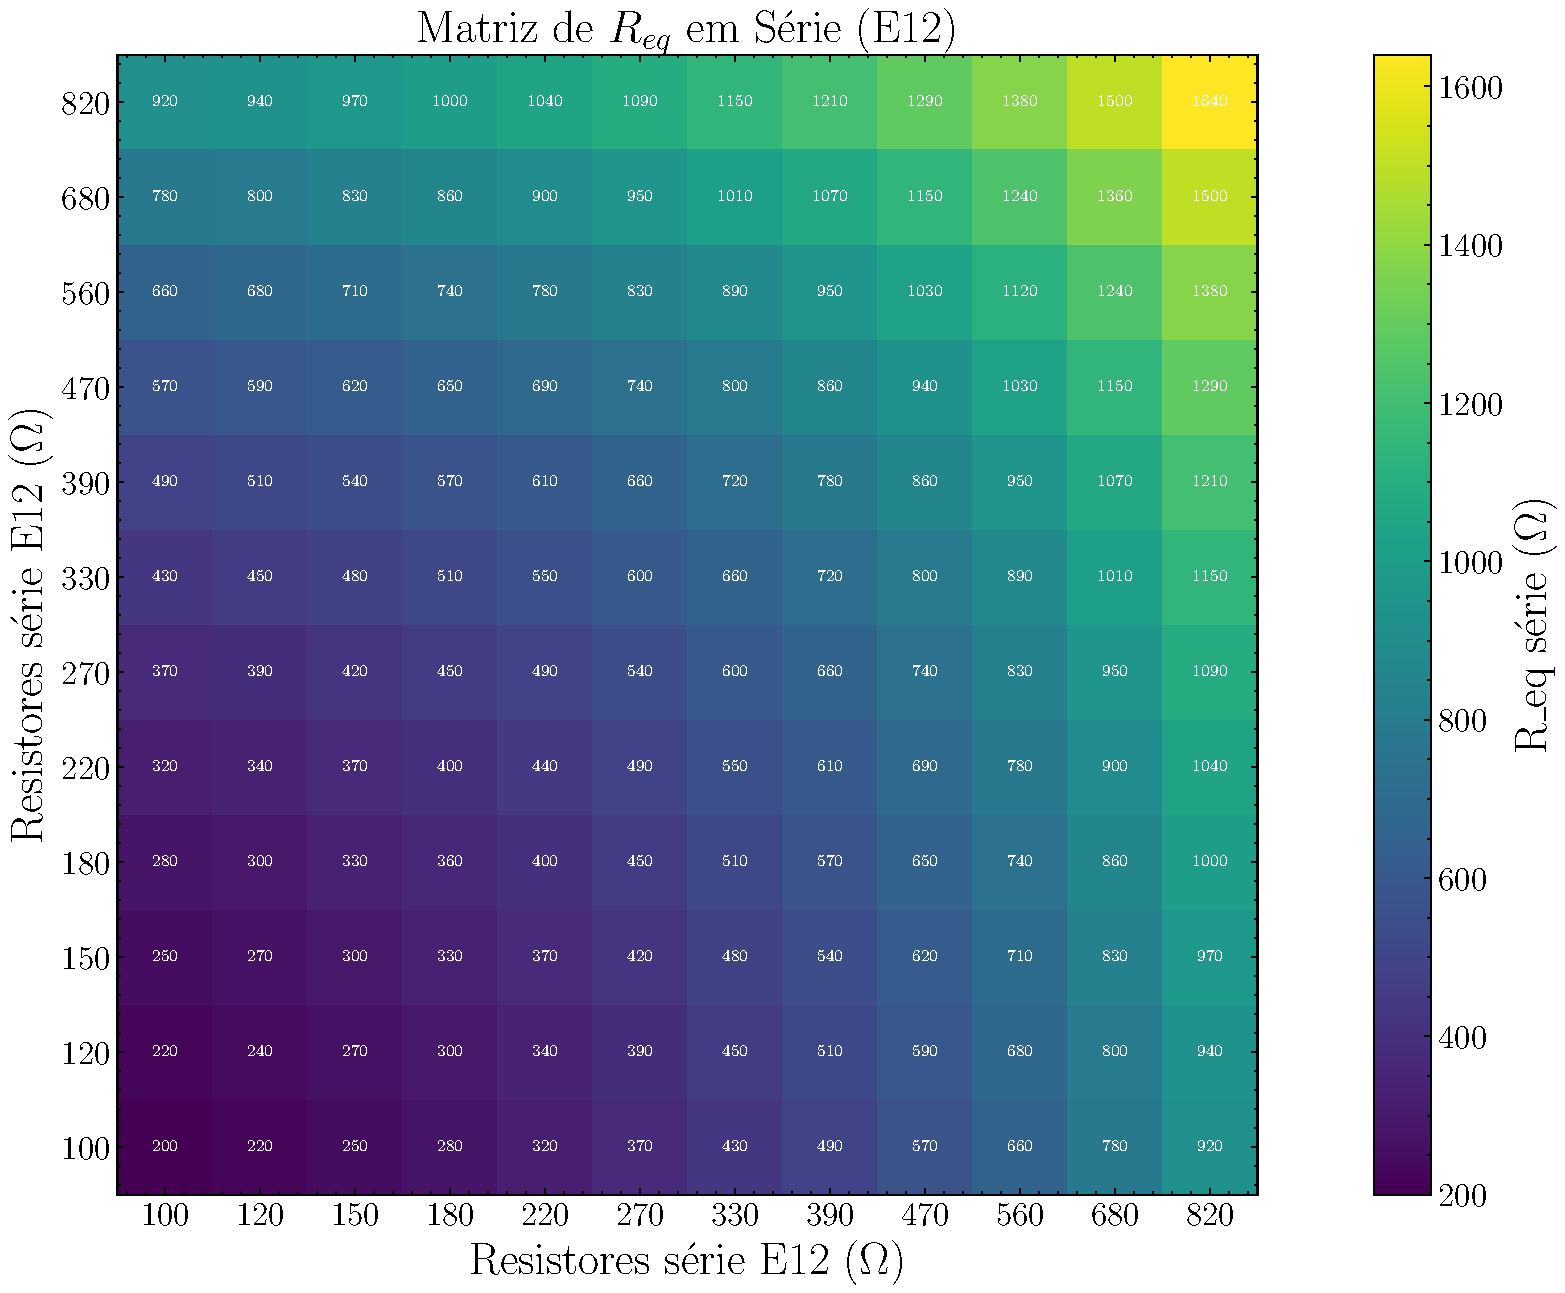
\includegraphics[width=0.8\linewidth]{figures/matriz_serie_e12.pdf}
\end{figure}

\begin{figure}[htbp]
    \centering
    \caption{Matriz de resistores em paralelo E12}
    \label{fig:matriz_paralelo_e12}
    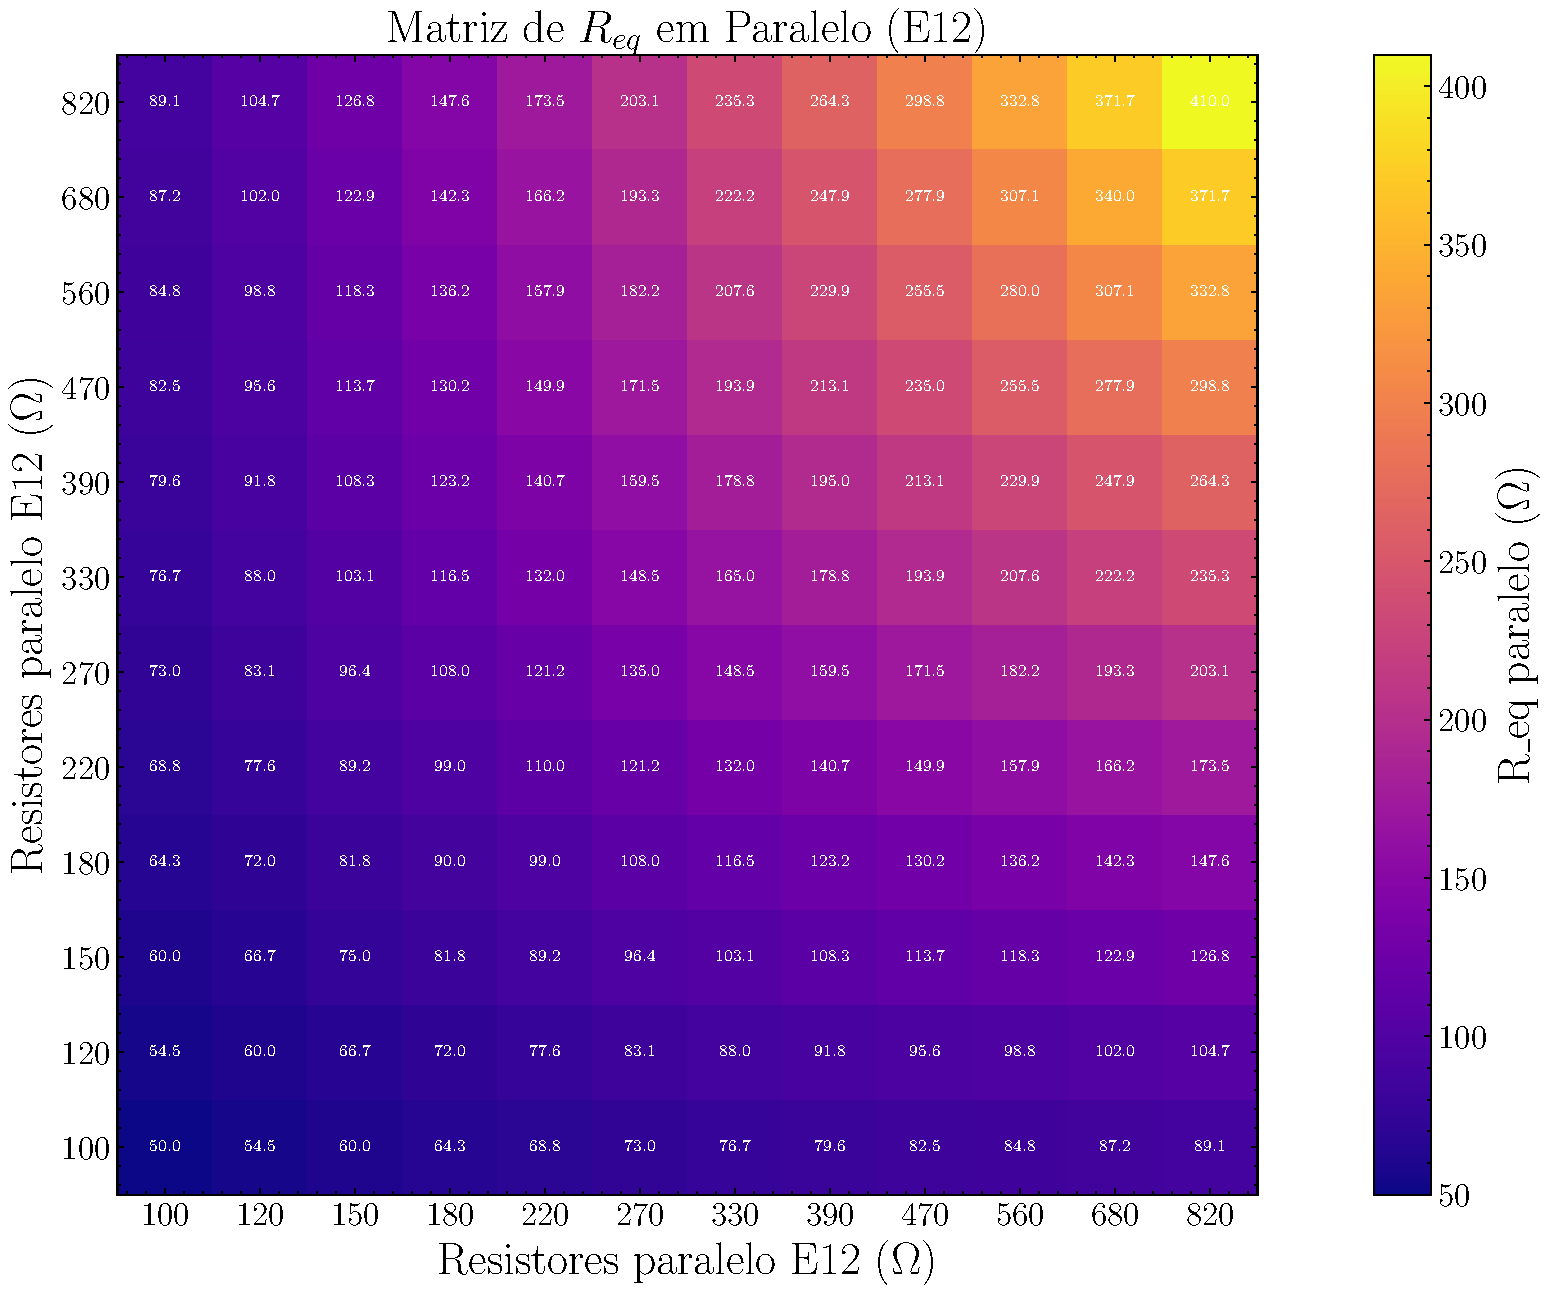
\includegraphics[width=0.8\linewidth]{figures/matriz_paralelo_e12.pdf}
\end{figure}

% \subsection{Série E12}

% A série E12 é uma das mais comuns e contempla valores padronizados de resistores amplamente utilizados em aplicações gerais. As figuras \ref{fig:matriz_paralelo_e12} e \ref{fig:matriz_serie_e12}  ilustram como os resistores dessa série podem ser combinados em série e paralelo, destacando os efeitos dessas associações na resistência equivalente. As cores representam


% \begin{figure}[htbp]
%     \centering
%     \caption{Matriz de resistores em série E12}
%     \label{fig:matriz_serie_e12}
%     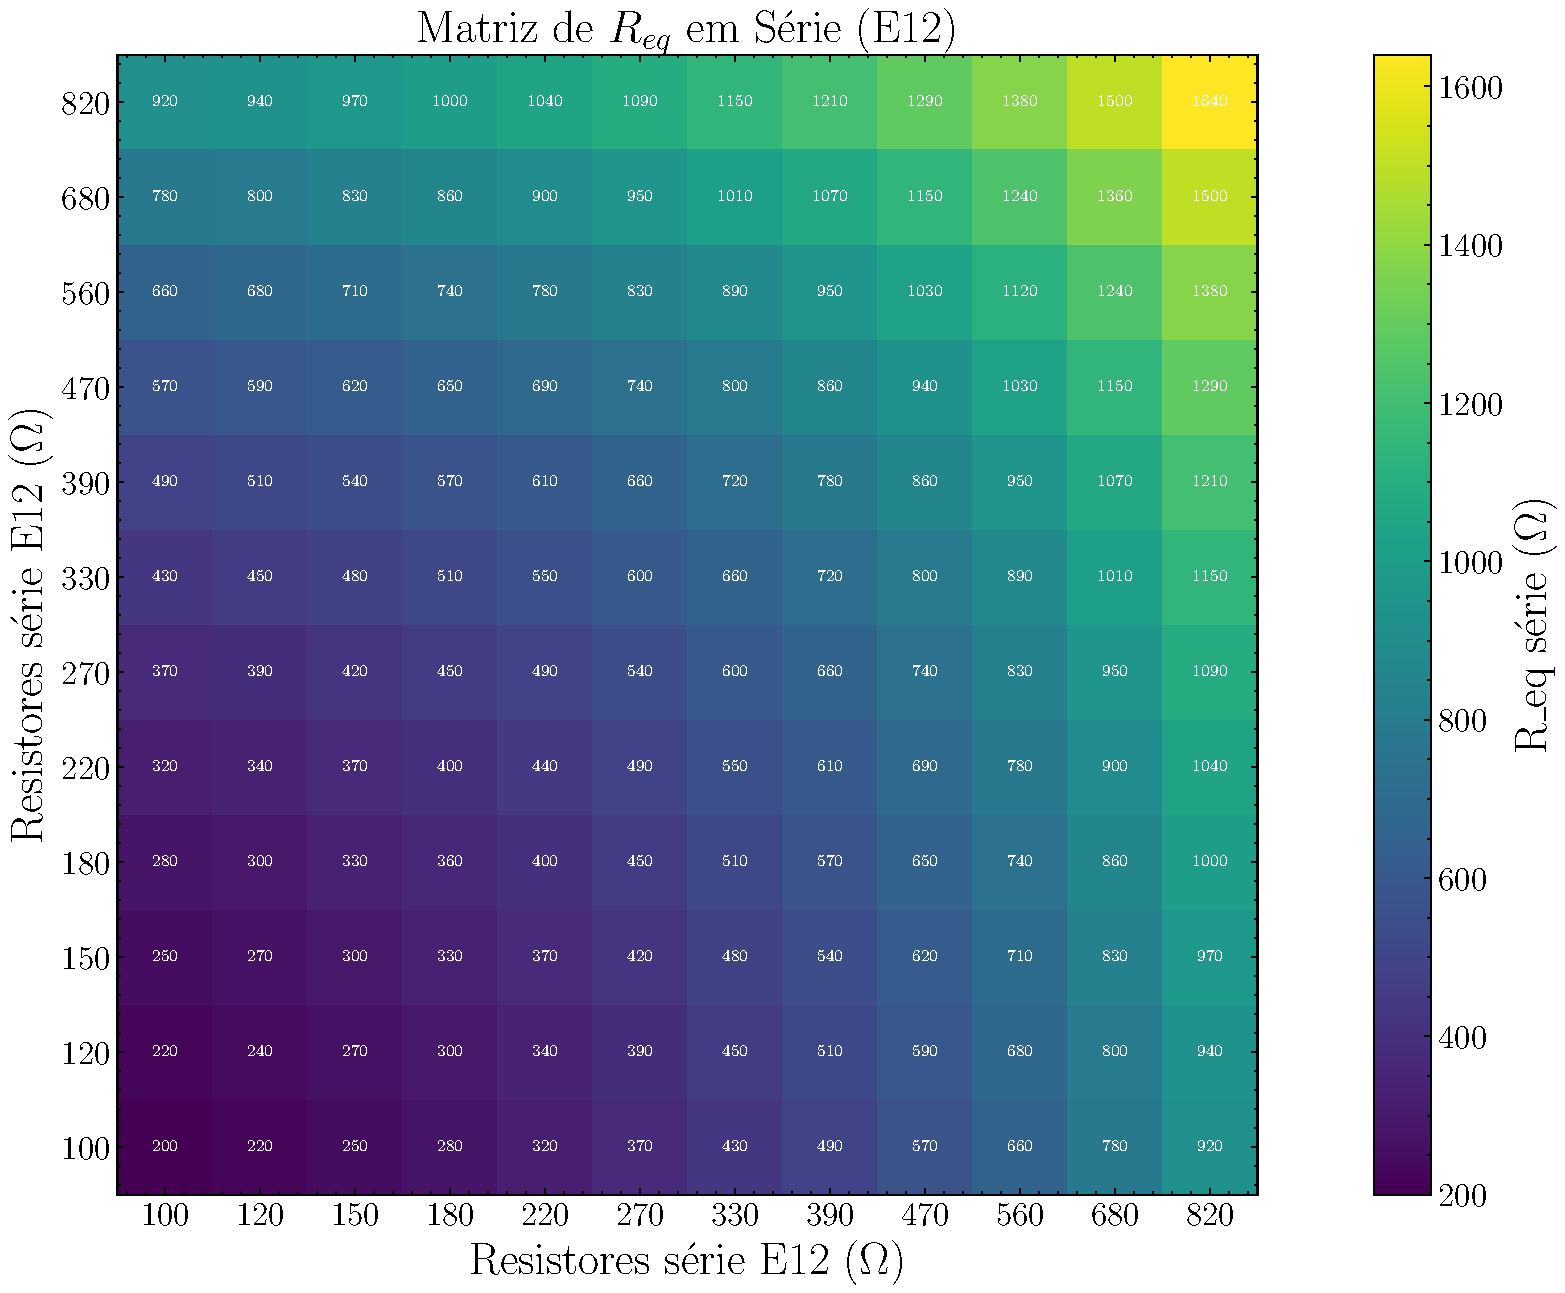
\includegraphics[width=0.8\linewidth]{figures/matriz_serie_e12.pdf}
% \end{figure}

% \begin{figure}[htbp]
%     \centering
%     \caption{Matriz de resistores em paralelo E12}
%     \label{fig:matriz_paralelo_e12}
%     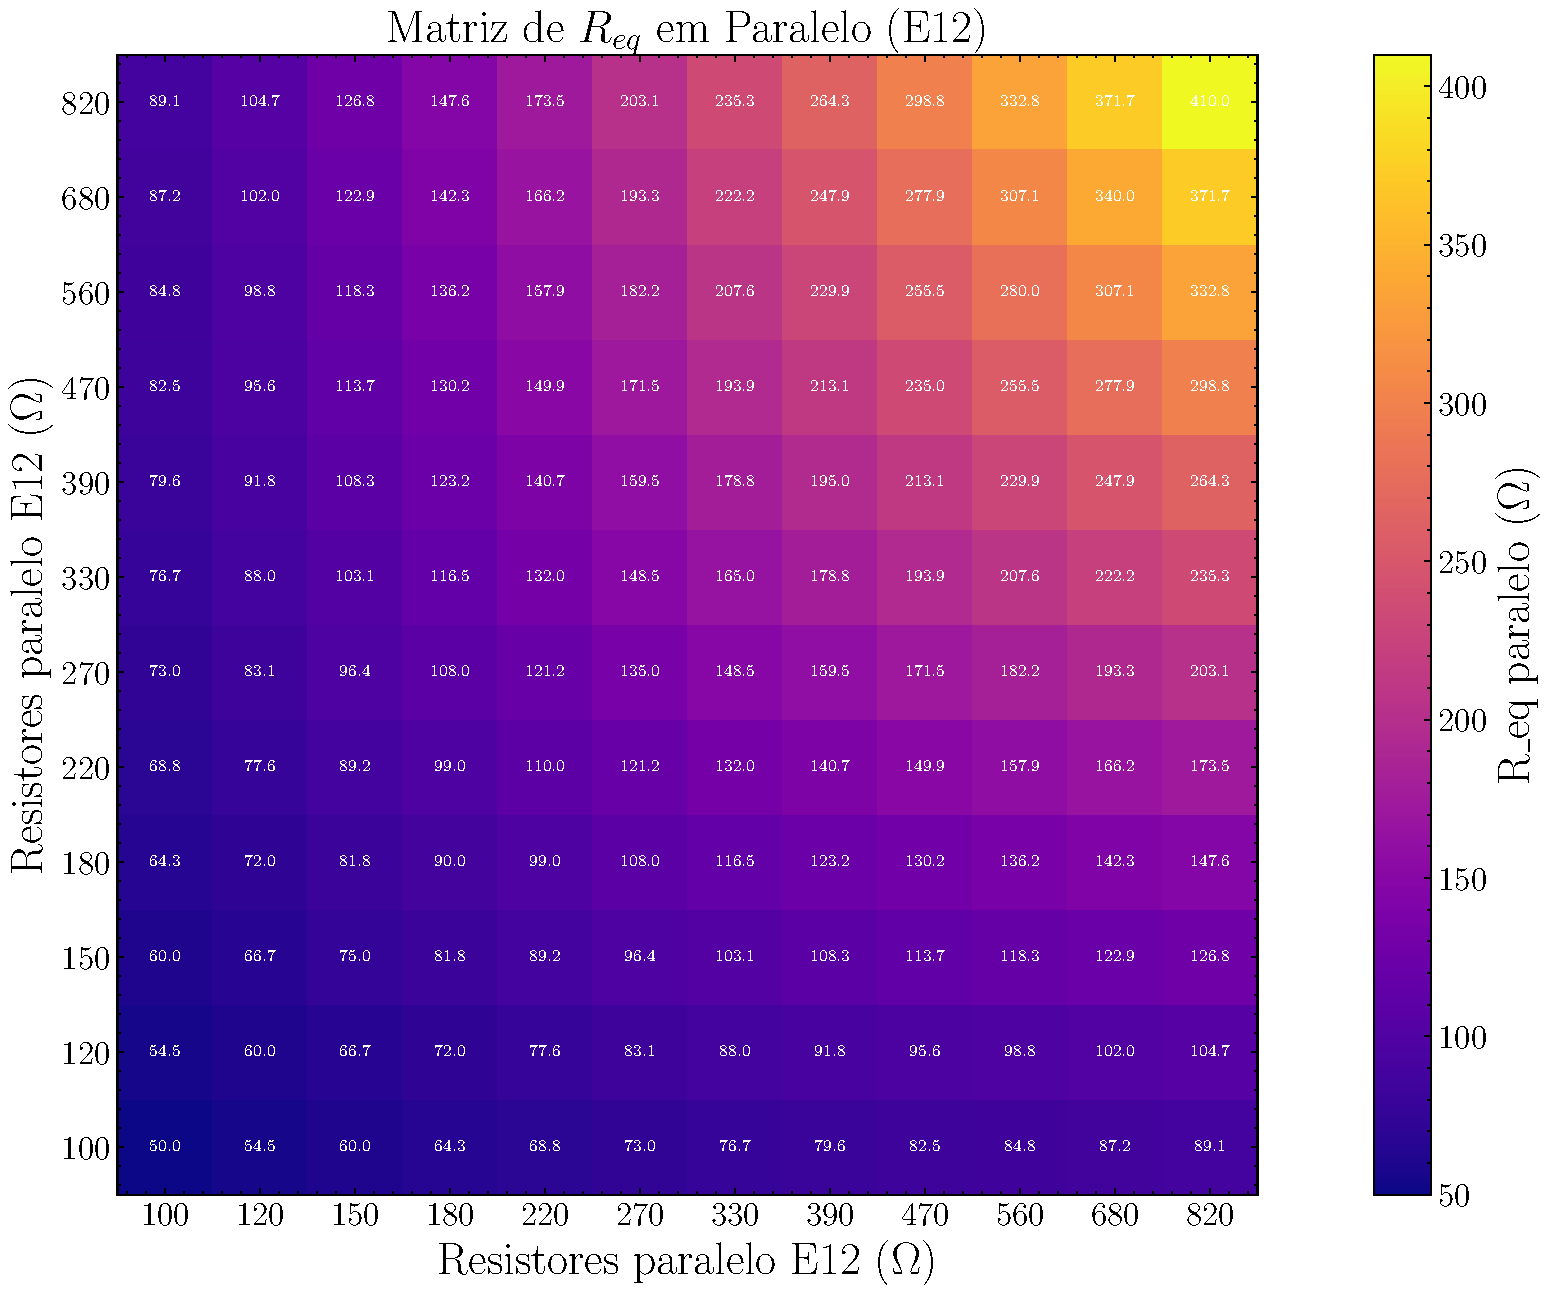
\includegraphics[width=0.8\linewidth]{figures/matriz_paralelo_e12.pdf}
% \end{figure}

% A associação em série resulta em uma resistência total maior, enquanto a associação em paralelo reduz a resistência equivalente.

\subsection{Série E24}

A série E24 é uma extensão da E12, oferecendo 24 valores nominais por década com espaçamento mais denso, o que permite maior precisão na seleção de resistores. Essa série é especialmente útil em aplicações que exigem tolerâncias mais estreitas, geralmente de 5%, e fornece uma resolução mais fina de valores dentro de cada ordem de grandeza \cite{iec60063}. Isso permite um controle mais preciso sobre os parâmetros de projeto em circuitos analógicos, filtros, divisores de tensão e ajustes de corrente.

A maior variedade de valores disponíveis na série E24 também amplia as possibilidades de combinação de resistores para alcançar resistências equivalentes próximas de alvos específicos. As Figuras~\ref{fig:matriz_serie_e24} e~\ref{fig:matriz_paralelo_e24} apresentam as matrizes resultantes das combinações em série e em paralelo entre dois resistores da série E24. Assim como na série E12, as cores representam os valores de resistência equivalente obtidos, evidenciando a distribuição e a densidade dos valores resultantes em cada tipo de associação.

A associação em série, ilustrada na Figura~\ref{fig:matriz_serie_e24}, amplia a gama de resistências possíveis ao somar os valores individuais, permitindo atingir faixas mais altas de resistência com maior precisão. Já a associação em paralelo, mostrada na Figura~\ref{fig:matriz_paralelo_e24}, permite reduzir a resistência equivalente de forma controlada, com benefícios adicionais no aumento da capacidade de corrente do circuito e na dissipação de potência distribuída entre os componentes.

A análise comparativa entre as séries E12 e E24, por meio dessas matrizes, destaca como a escolha da série afeta diretamente a flexibilidade de projeto. A série E24, por conter o dobro de valores por década, permite combinações mais ajustadas aos requisitos desejados, tornando-se uma opção vantajosa em projetos que demandam maior precisão sem recorrer a componentes especiais ou de difícil aquisição.


\begin{figure}[htbp]
    \centering
    \caption{Matriz de resistores em série E24}
    \label{fig:matriz_serie_e24}
    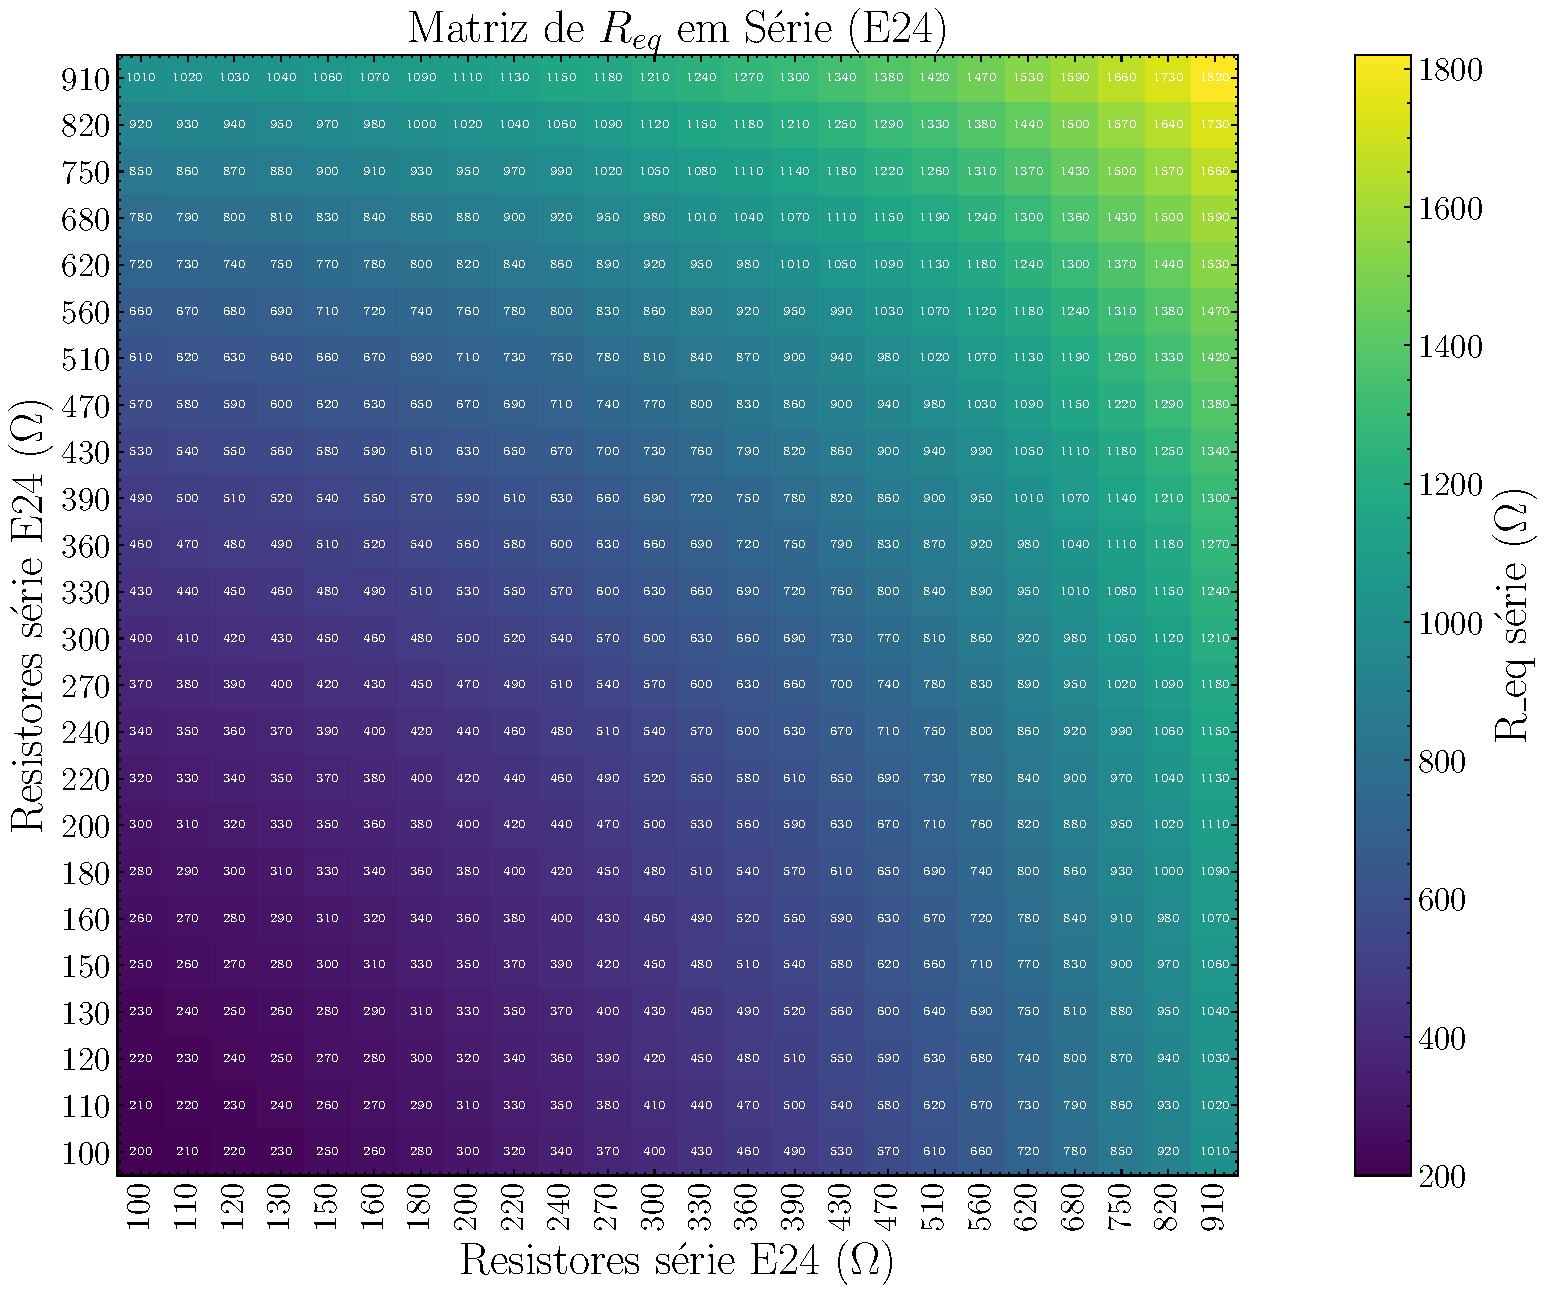
\includegraphics[width=0.8\linewidth]{figures/matriz_serie_e24.pdf}
\end{figure}

\begin{figure}[htbp]
    \centering
    \caption{Matriz de resistores em paralelo E24}
    \label{fig:matriz_paralelo_e24}
    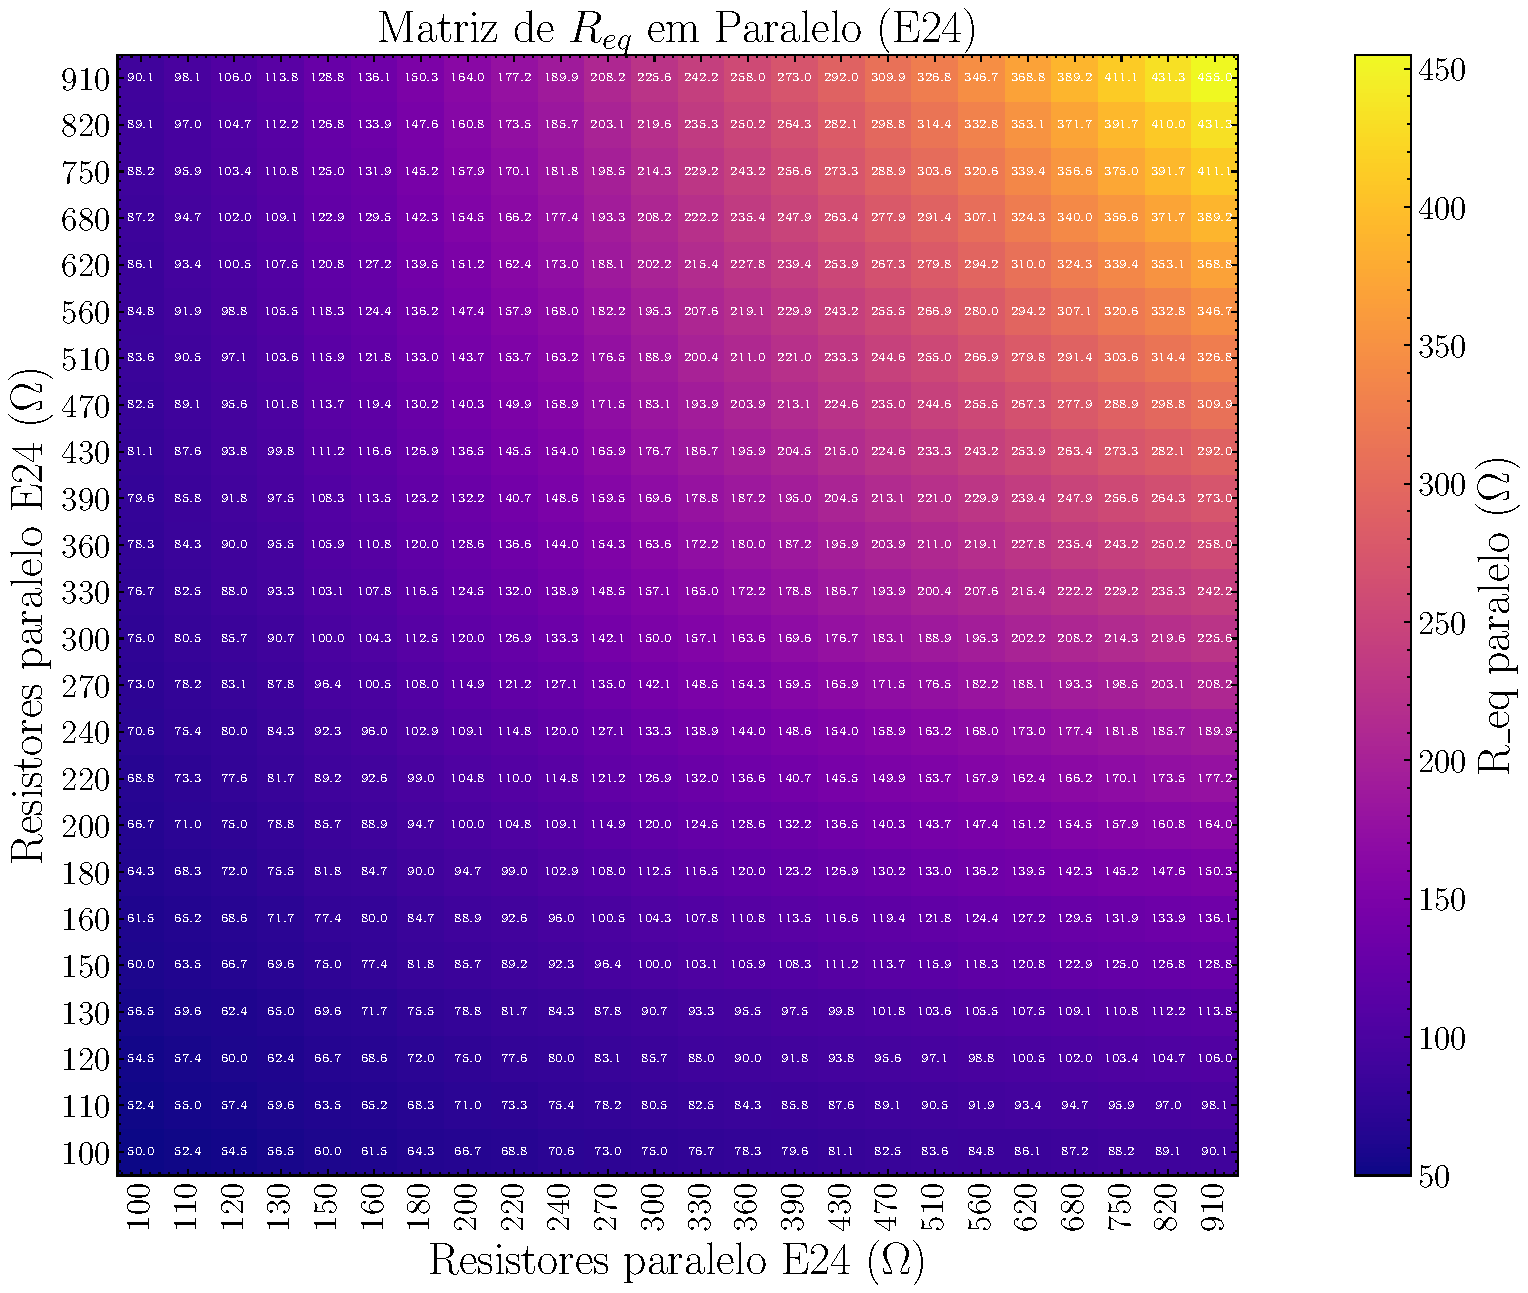
\includegraphics[width=0.8\linewidth]{figures/matriz_paralelo_e24.pdf}
\end{figure}

% \subsection{Série E24}

% A série E24 oferece maior granularidade de valores comerciais, permitindo combinações ainda mais precisas para projetos eletrônicos. As associações possíveis são exemplificadas nas figuras a seguir:
% \begin{figure}[htbp]
%     \centering
%     \caption{Matriz de resistores em série E24}
%     \label{fig:matriz_serie_e24}
%     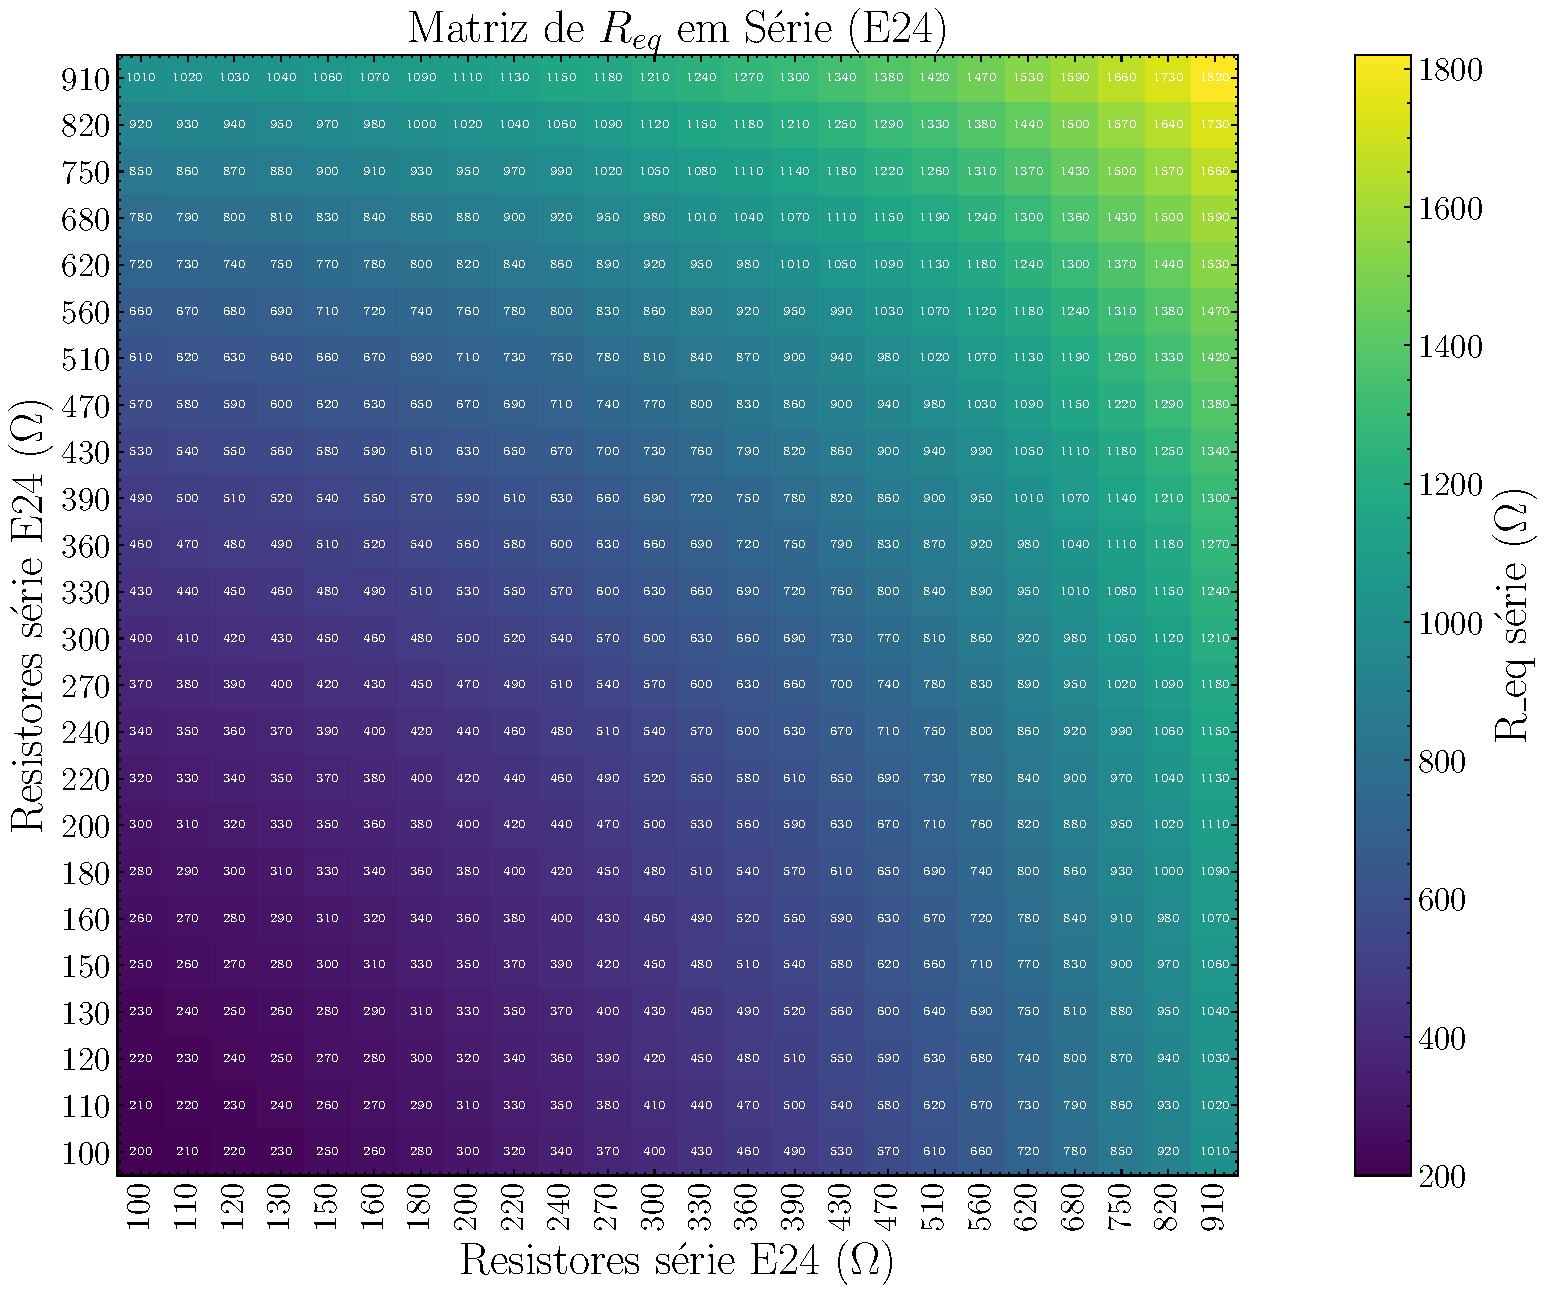
\includegraphics[width=0.8\linewidth]{figures/matriz_serie_e24.pdf}
% \end{figure}

% \begin{figure}[htbp]
%     \centering
%     \caption{Matriz de resistores em paralelo E24}
%     \label{fig:matriz_paralelo_e24}
%     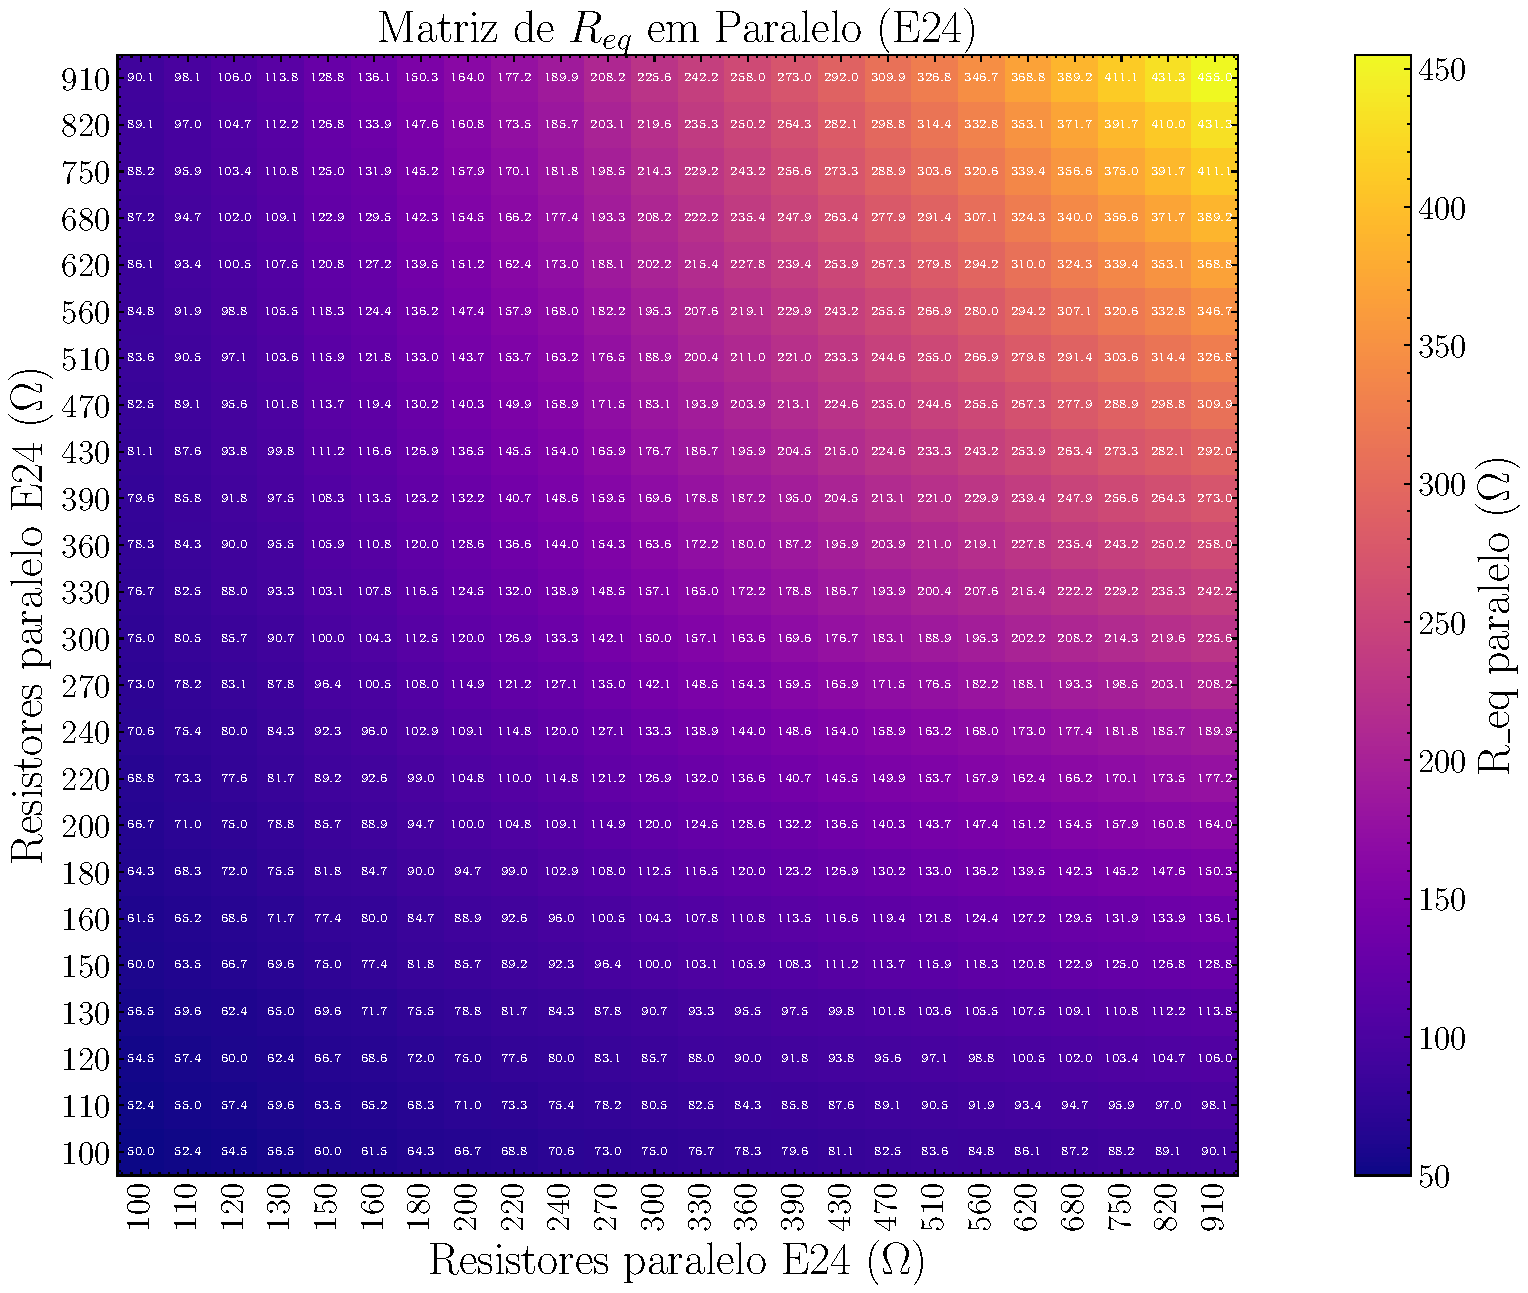
\includegraphics[width=0.8\linewidth]{figures/matriz_paralelo_e24.pdf}
% \end{figure}


% Essas associações demonstram como a escolha da série influencia a flexibilidade de valores alcançáveis em um projeto.

\section{Materiais e Métodos}

O experimento foi conduzido utilizando os seguintes materiais:

\begin{itemize}
    \item 10 resistores de $1,k\Omega$ com tolerância de 5%;
    \item 10 resistores de $1,M\Omega$ com tolerância de 5%;
    \item Fonte de alimentação de corrente contínua (CC);
    \item Multímetro digital de três dígitos;
    \item Protoboard e cabos de conexão;
    \item Resistor de aquecimento de $1000,\text{W}$ (220,VAC) para simulação do efeito Joule.
\end{itemize}

Os valores nominais dos resistores utilizados foram verificados individualmente com o multímetro digital, respeitando a tolerância de 5\% indicada pelos fabricantes. Esse parâmetro representa a variação admissível entre o valor real do componente e o valor nominal, o que introduz um erro de leitura que deve ser considerado na análise dos resultados. Além disso, a precisão limitada do multímetro (com resolução de $0.1~\Omega$ para a faixa de baixa resistência) também contribui para o erro experimental associado às medições.

Foram montados circuitos resistivos com diferentes configurações: associações em série, em paralelo e mistas, utilizando protoboard para facilitar a montagem sem a necessidade de solda. Em cada configuração, foram realizadas medições de resistência total, tensão e corrente elétrica por meio do multímetro digital. Os dados obtidos foram utilizados para comparar os resultados experimentais com os valores teóricos previstos pelas equações das associações de resistores.

Adicionalmente, foi realizado um experimento demonstrativo do efeito Joule, com o objetivo de ilustrar a conversão de energia elétrica em energia térmica. Para isso, utilizou-se um resistor de aquecimento de $1000,\text{W}$ alimentado por tensão alternada (220V). O resistor foi submerso em 500mL de água em temperatura ambiente (25°C), e a temperatura foi monitorada ao longo do tempo até atingir a temperatura de ebulição da água. O experimento permite observar, qualitativamente, a dissipação de potência elétrica como calor, de acordo com a relação $P=R\cdot I^2$, onde $P$ é a potência dissipada, $R$ é a resistência do resistor e $I$ é a corrente elétrica que passa por ele.

A Figura~\ref{fig:montagem_aquecimento} mostra a montagem experimental do sistema para observação do efeito Joule.

% TODO: adicionar fotos das montagens 
% \begin{figure}[htbp]
%     \centering
%     \caption{Montagem dos circuitos resistivos em protoboard}
%     \label{fig:montagem_resistores}
%     \includegraphics[width=0.8\linewidth]{figures/montagem_resistores.jpg}
% \end{figure}

\begin{figure}[htbp]
    \centering
    \caption{Montagem do experimento do efeito Joule}
    \label{fig:montagem_aquecimento}
    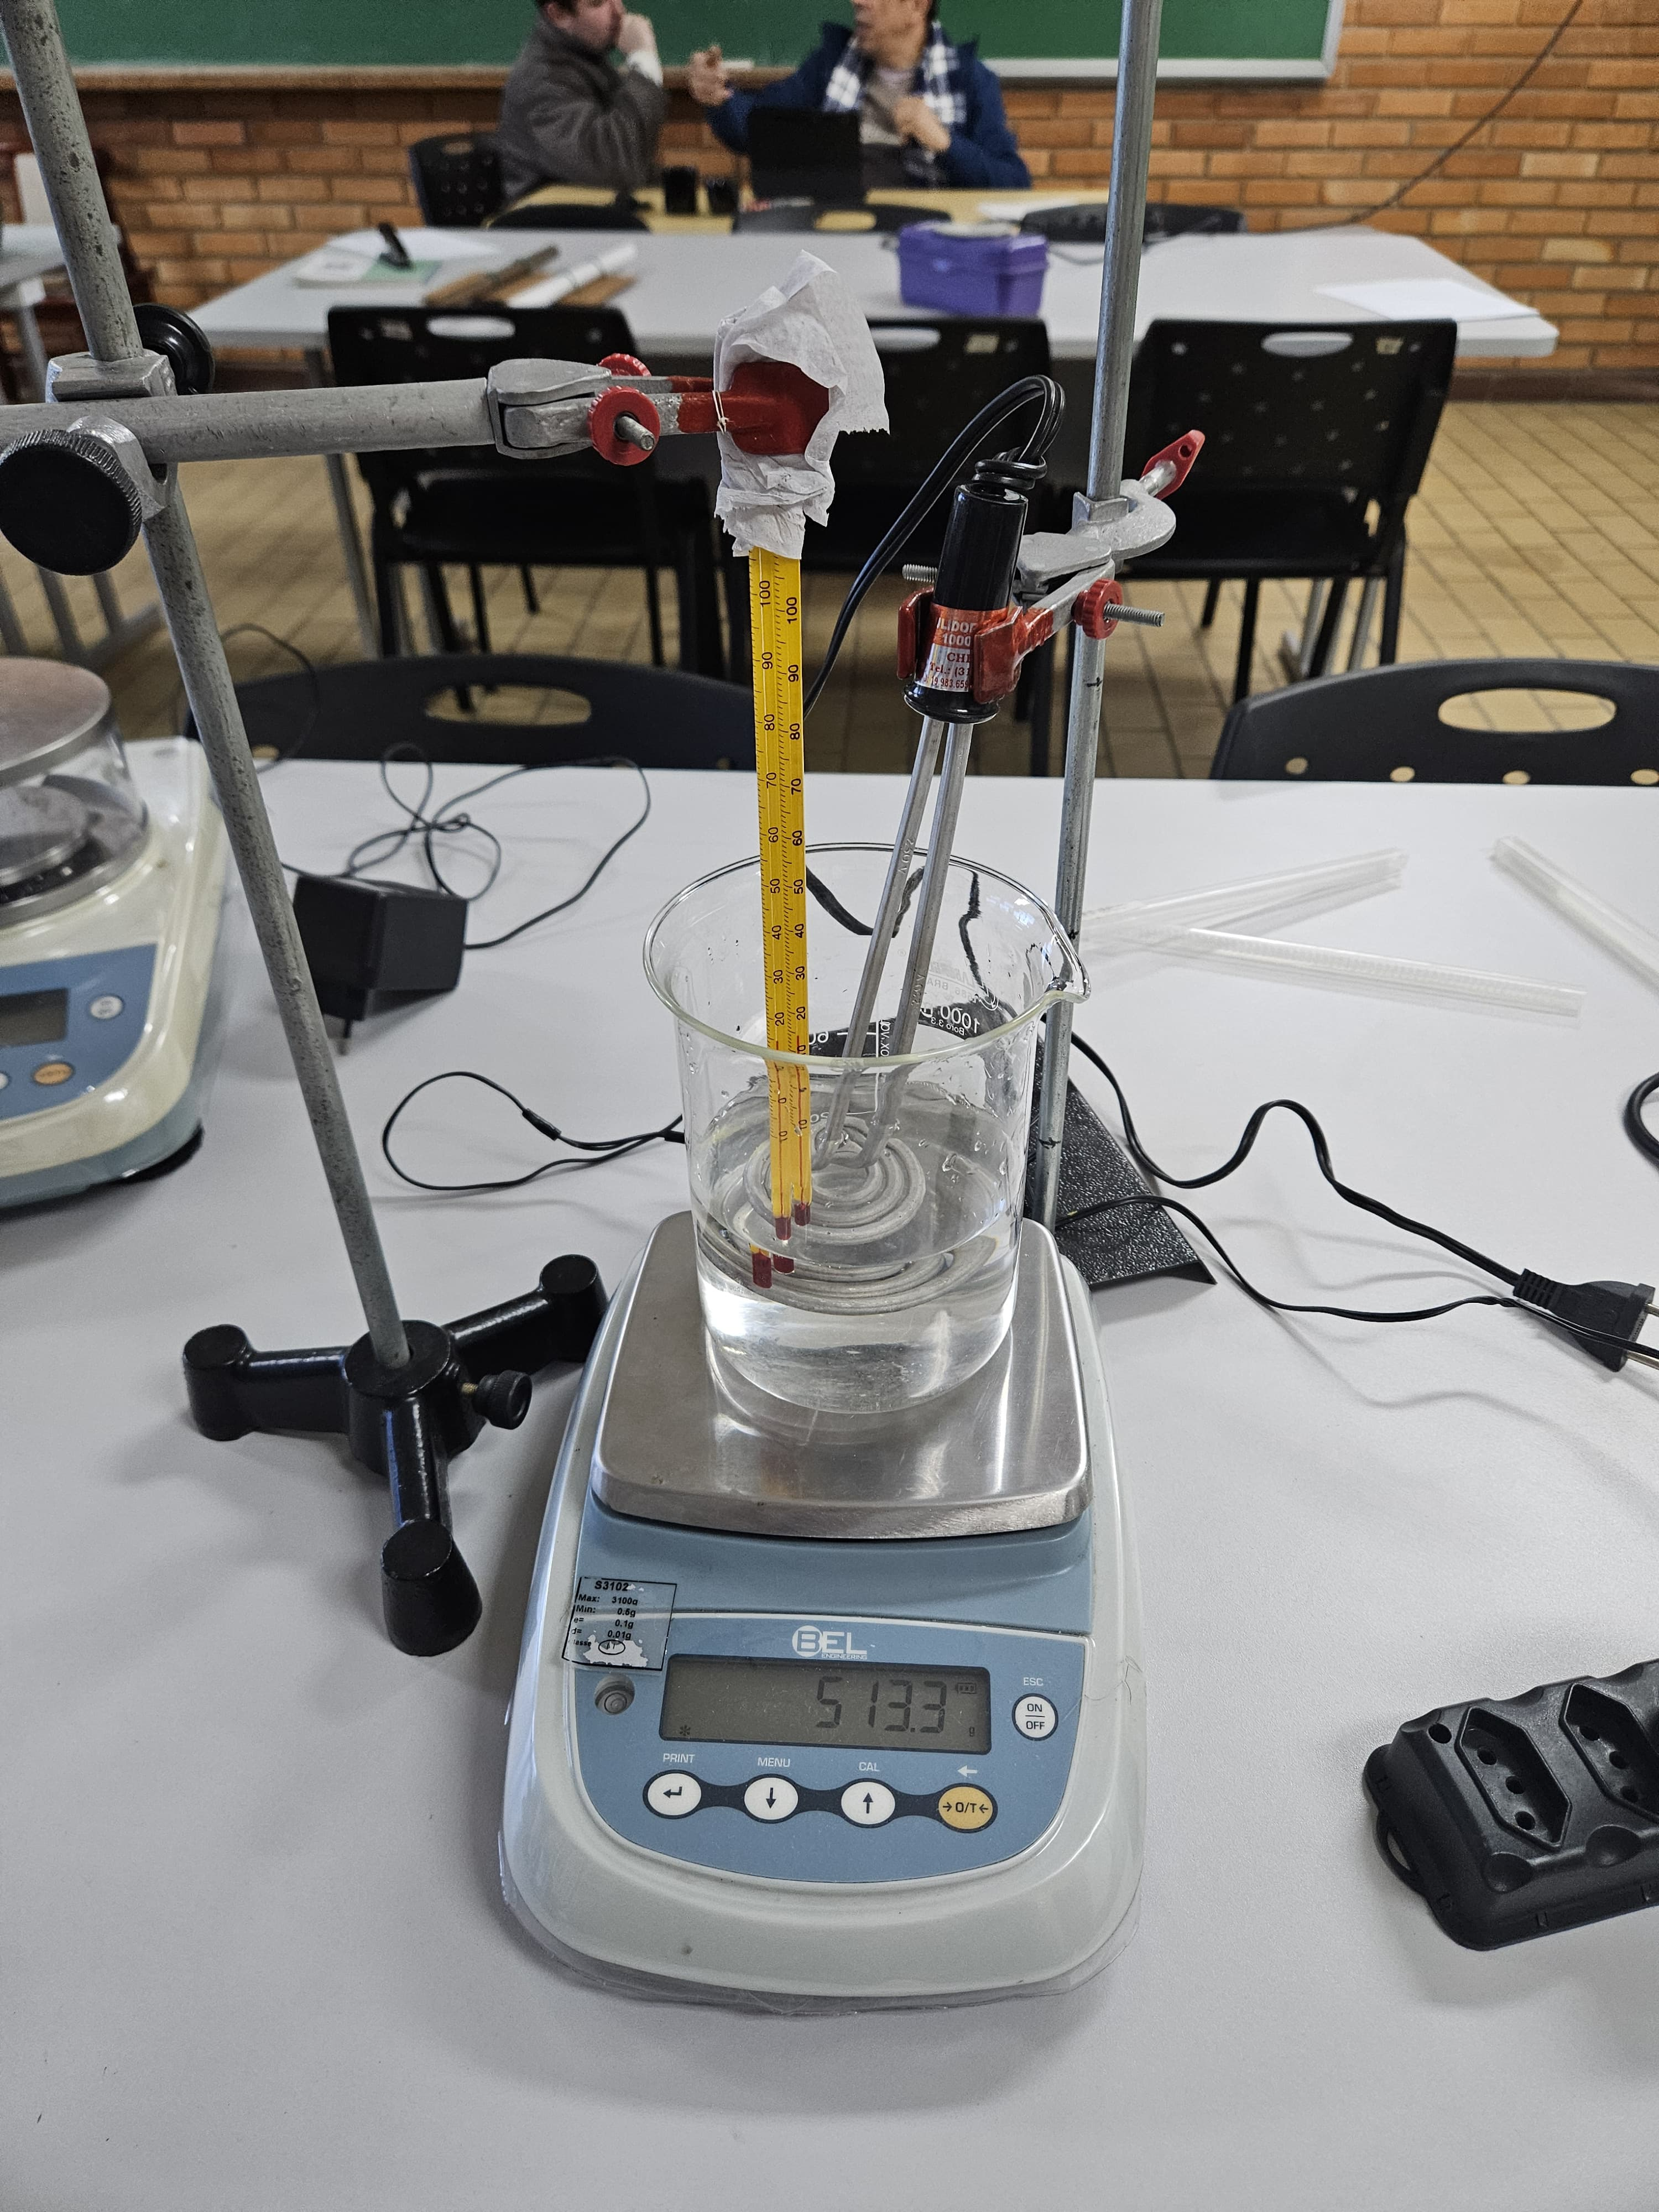
\includegraphics[width=0.8\linewidth]{figures/montagem_aquecimento.jpeg}
\end{figure}



% \section{Materiais e métodos}

% \begin{itemize}
%     \item 10 resistores de $1k\Omega$ % [COMENTARIO PROFESSOR] e a tolerrancia (erro na leitura real das medidas)
%           % [COMENTARIO PROFESSOR] erro de leitura das medidas que podemos ter ou aceitar nos resistores
%     \item 10 resistores de $1M\Omega$
%     \item Fonte de alimentação CC
%     \item Multímetro digital
%     \item Protoboard e cabos
%     \item Resistor de aquecimento 1000W (220VAC) para simulação do efeito Joule
% \end{itemize}

% Foram montados circuitos com resistores em série, paralelo e mista. As medições de resistência, tensão e corrente foram realizadas com o multímetro digital. O protoboard facilita a montagem dos circuitos sem a necessidade de solda.

% Para simular o efeito Joule, foi utilizado um resistor de aquecimento 1000W (220VAC) submerso em 500mL de água, com a temperatura ambiente de 25°C, e foi monitorada a temperatura da água ao longo do tempo até a temperatura de evaporação.

% % adicionar fotos das montagens \ref{fig:montagem_resistores} e \ref{fig:montagem_efeito_joule}

\section{Associação de resistores}

\subsection{Distribuição normal dos valores medidos}

A análise estatística dos valores medidos permite determinar a média, desvio padrão e erro médio dos resistores:

Média

\begin{equation}
    R = \frac{1}{n} \sum_{i=1}^{n} R_i,
\end{equation}

\noindent
Onde $R$ é a média e $n$ o número de resistores.

Desvio padrão:

\begin{equation}
    \sigma = \sqrt{\frac{1}{n-1} \sum_{i=1}^{n} (R_i - R)^2},
\end{equation}

\noindent
Onde $\sigma$ representa a dispersão dos valores em relação à média.

Erro médio:

\begin{equation}
    \sigma_n = \frac{\sigma}{\sqrt{n}},
\end{equation}

\noindent
Onde $\sigma_n$ é o erro médio, $\sigma$ é o desvio padrão e $n$ é o número de resistores.

\begin{figure}[htbp]
    \centering
    \caption{Distribuição normal dos valores medidos}
    \label{fig:plot_hist_1k}
    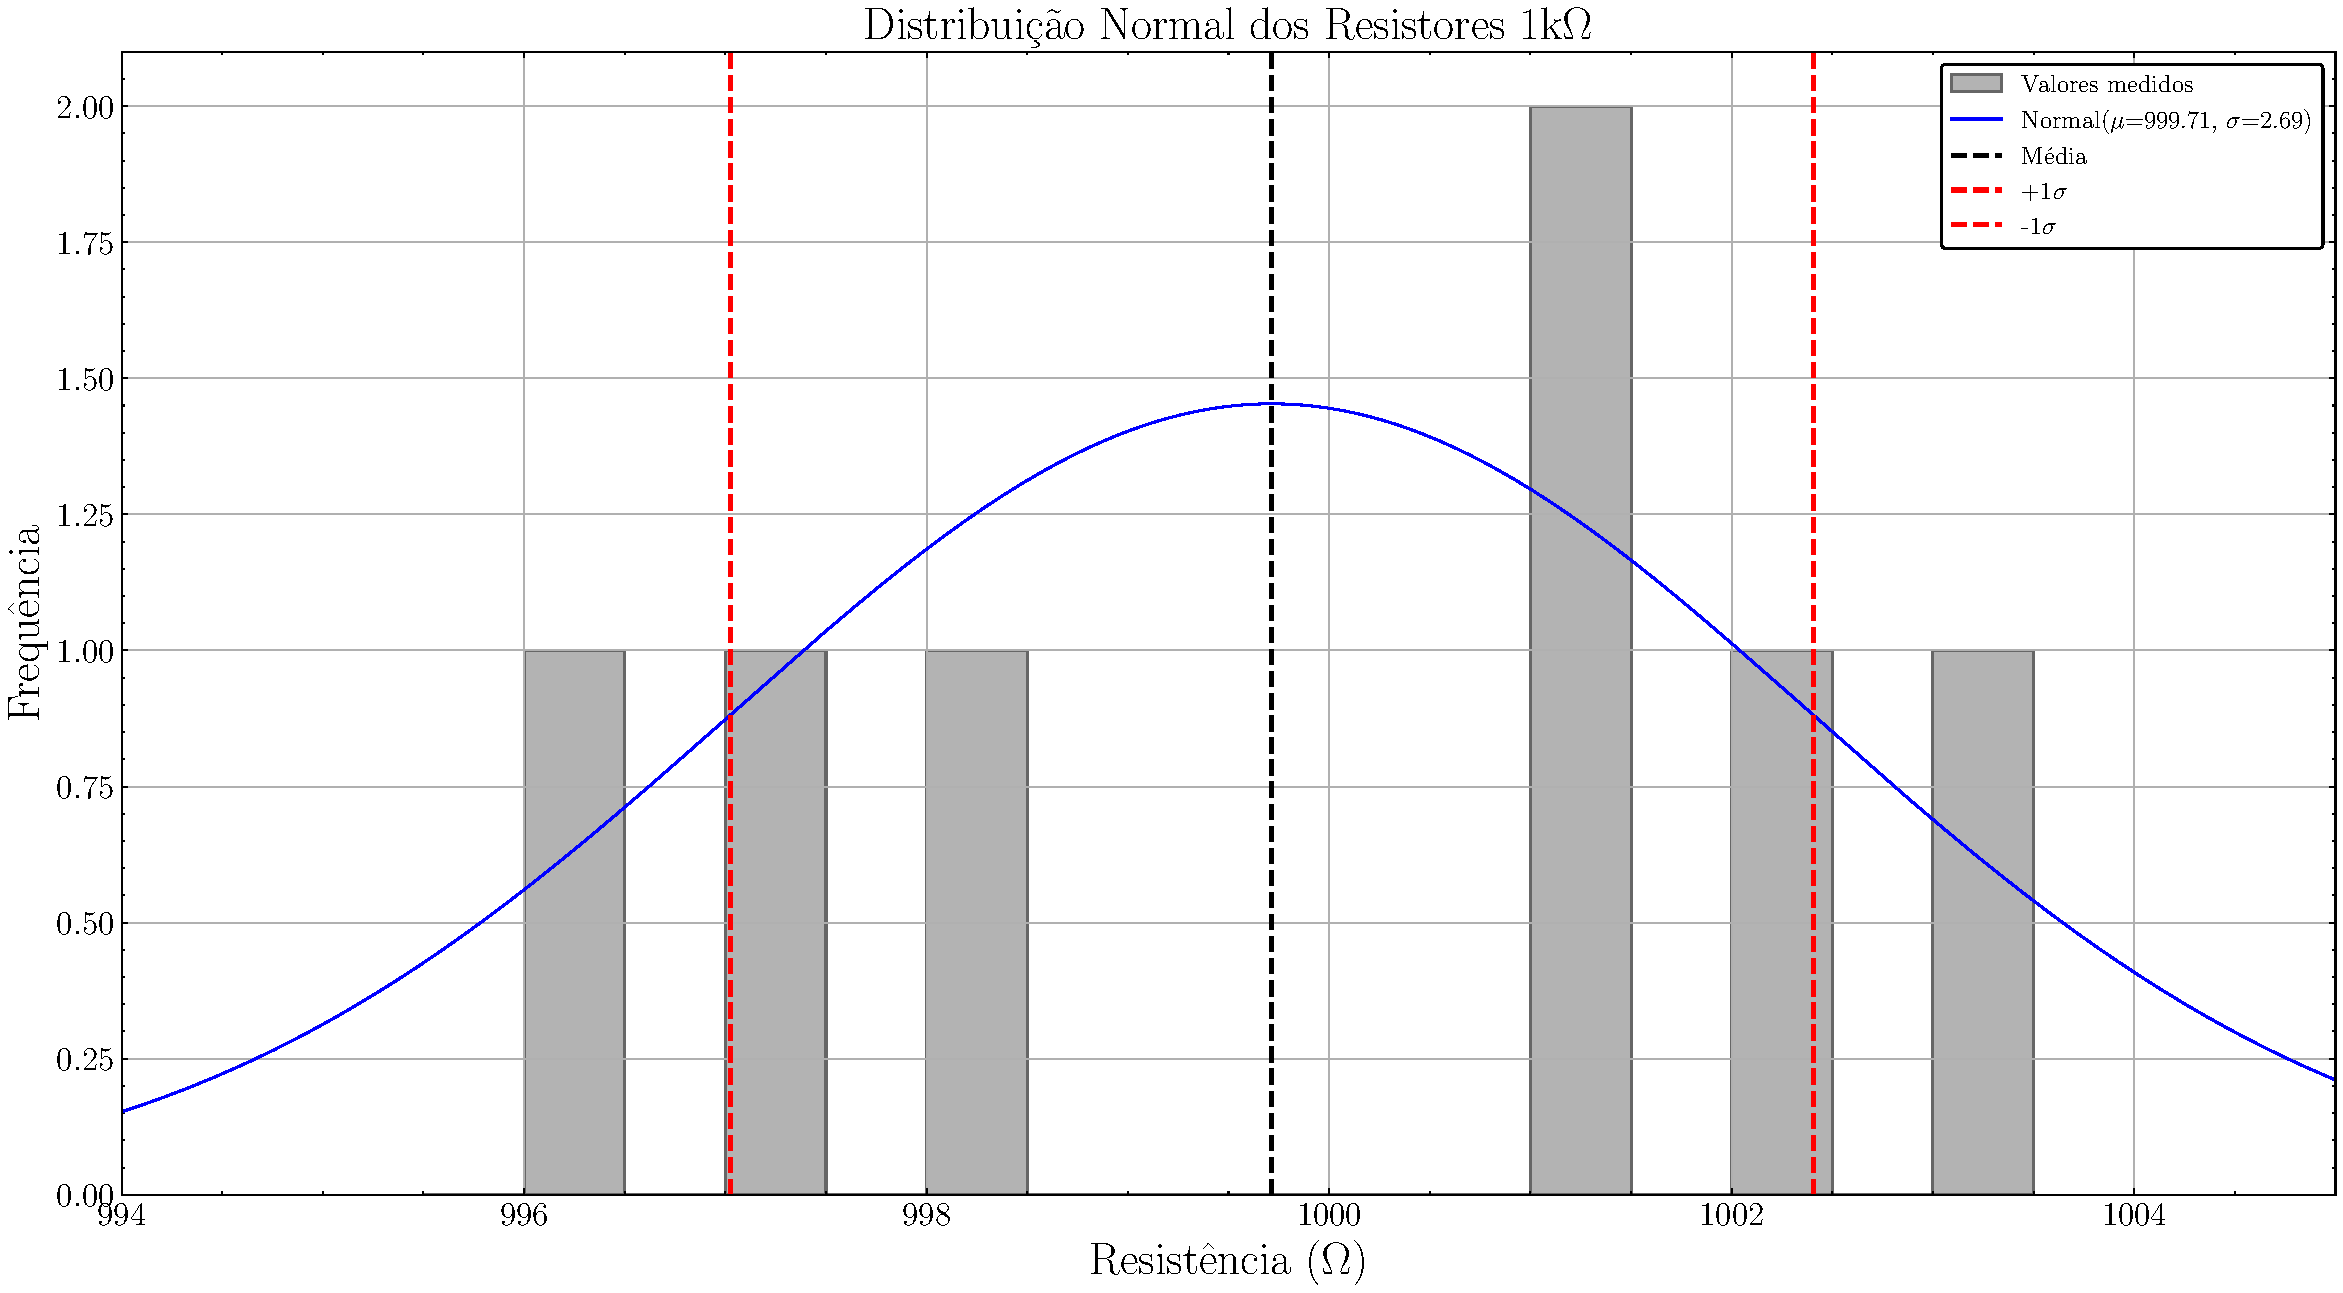
\includegraphics[width=0.8\linewidth]{figures/plot_hist_1k.pdf}
\end{figure}

\subsection{Associação de resistores (série, paralelo e mista)}

O erro absoluto na associação em série pode ser obtido por meio da soma das incertezas individuais:

\begin{equation}
    \sigma_{n_{eq}} = \sum_{i=1}^{n} \sigma_{n_i},
\end{equation}

\noindent
Onde $\sigma_{n_{eq}}$ é a incerteza total da associação em série e $\sigma_{n_i}$ são as incertezas individuais de cada resistor.

A propagação de erro para a associação em paralelo é dada por:

\begin{equation}
    \sigma_{n_{eq}} = R_{eq}^2 \sqrt{\sum_{i=1}^{n} \left(\frac{\sigma_{n_i}}{R_i^2}\right)^2},
\end{equation}

\noindent
Onde \(\sigma_{n_{eq}}\) é a incerteza total da associação em paralelo; \(\sigma_{n_i}\) são as incertezas individuais de cada resistor; e \(R_{eq}\) é a resistência equivalente do conjunto.

A resistência equivalente de um circuito misto pode ser representada, por exemplo, da seguinte forma:

\begin{align*}
    \begin{split}
        R_{eq} & = 1k\Omega + \left(1M\Omega \parallel 1k\Omega\right) + \left(1M\Omega \parallel 1M\Omega\right) \\
               & + \left(1k\Omega \parallel 1k\Omega\right) + 1M\Omega
    \end{split}
\end{align*}

\noindent
Onde o operador $\parallel$ indica a associação em paralelo entre dois resistores, cujo valor equivalente pode ser calculado por:

\begin{equation}
    R_{eq} = \left( \frac{1}{R_1} + \frac{1}{R_2} \right)^{-1}
\end{equation}

\begin{figure}[htbp]
    \centering
    \caption{Cálculo das resistências do circuito misto}
    \label{fig:plot_assoc_mista}
    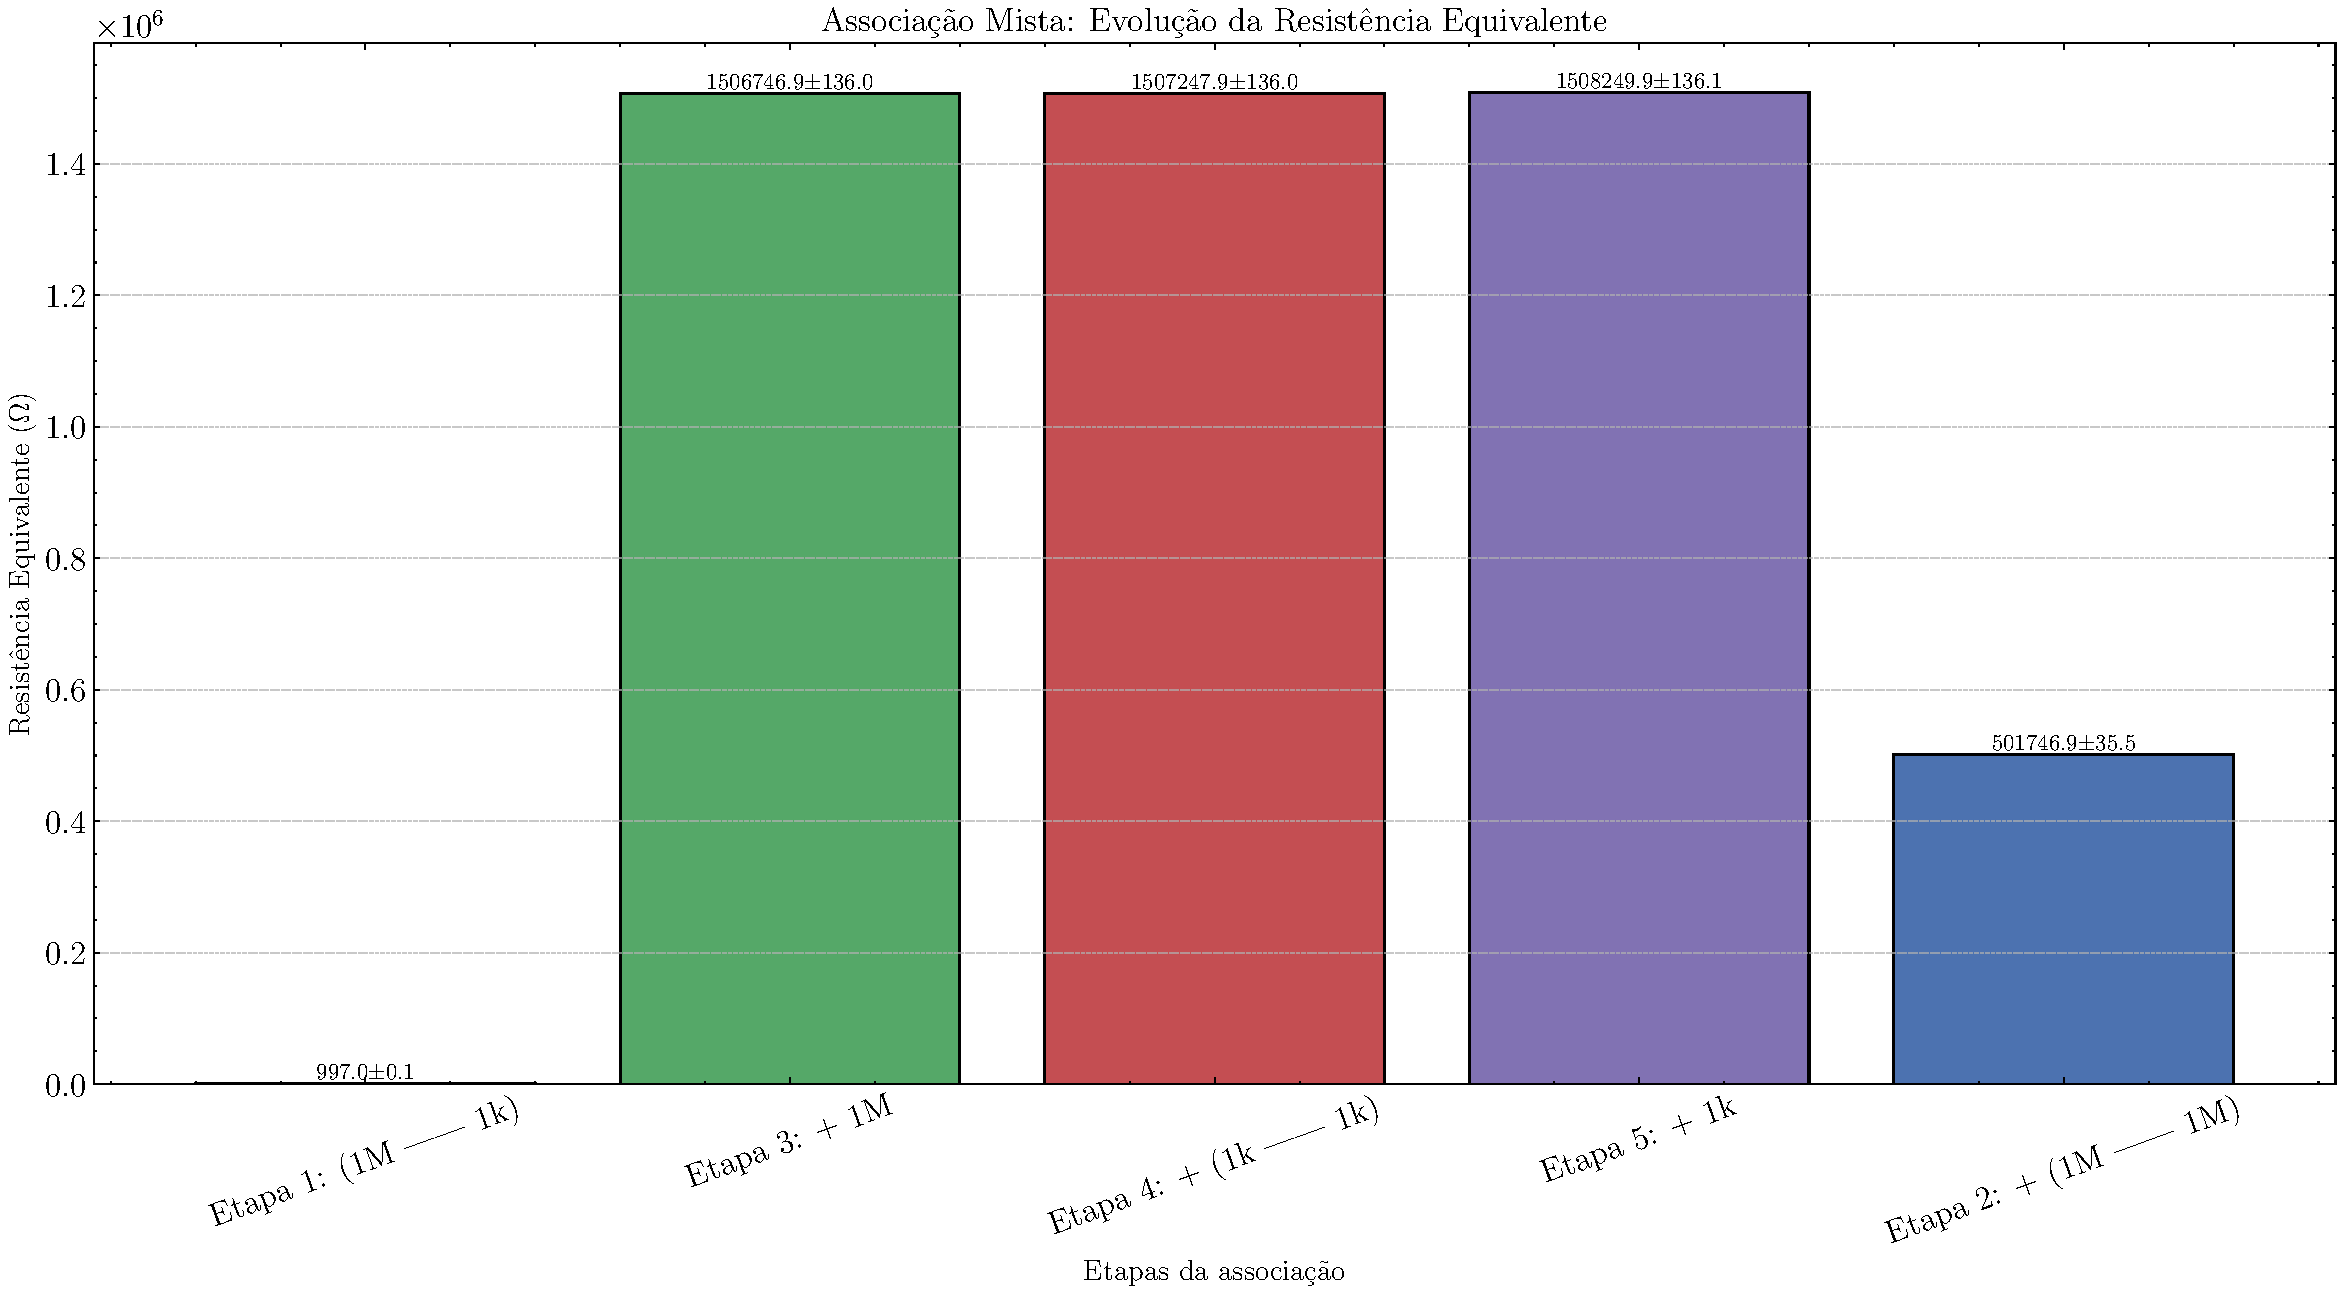
\includegraphics[width=0.8\linewidth]{figures/plot_assoc_mista.pdf}
\end{figure}


% \section{Associação de resistores}

% \subsection{Distribuição normal dos valores medidos}

% A análise estatística dos valores medidos permite determinar a média, desvio padrão e erro médio dos resistores:

% Média

% \begin{equation}
%     R = \frac{1}{n} \sum_{i=1}^{n} R_i,
% \end{equation}

% \noindent
% Onde $R$ é a média $n$ o número de resistores.

% Desvio padrão:

% \begin{equation}
%     \sigma = \sqrt{\frac{1}{n-1} \sum_{i=1}^{n} (R_i - R)^2},
% \end{equation}

% \noindent
% Onde $sigma$ representa a dispersão dos valores em relação à média.

% Erro médio

% \begin{equation}
%     \sigma_n = \frac{\sigma}{\sqrt{n}}, % [COMENTARIO PROFESSOR] deveira ser \sigma_n não \sigma_n
% \end{equation}

% \noindent
% Onde $\sigma_n$ é o erro médio $sigma$ é o desvio padrão $n$ é o número de resistores.

% \begin{figure}[htbp]
%     \centering
%     \caption{Distribuição normal dos valores medidos}
%     \label{fig:plot_hist_1k}
%     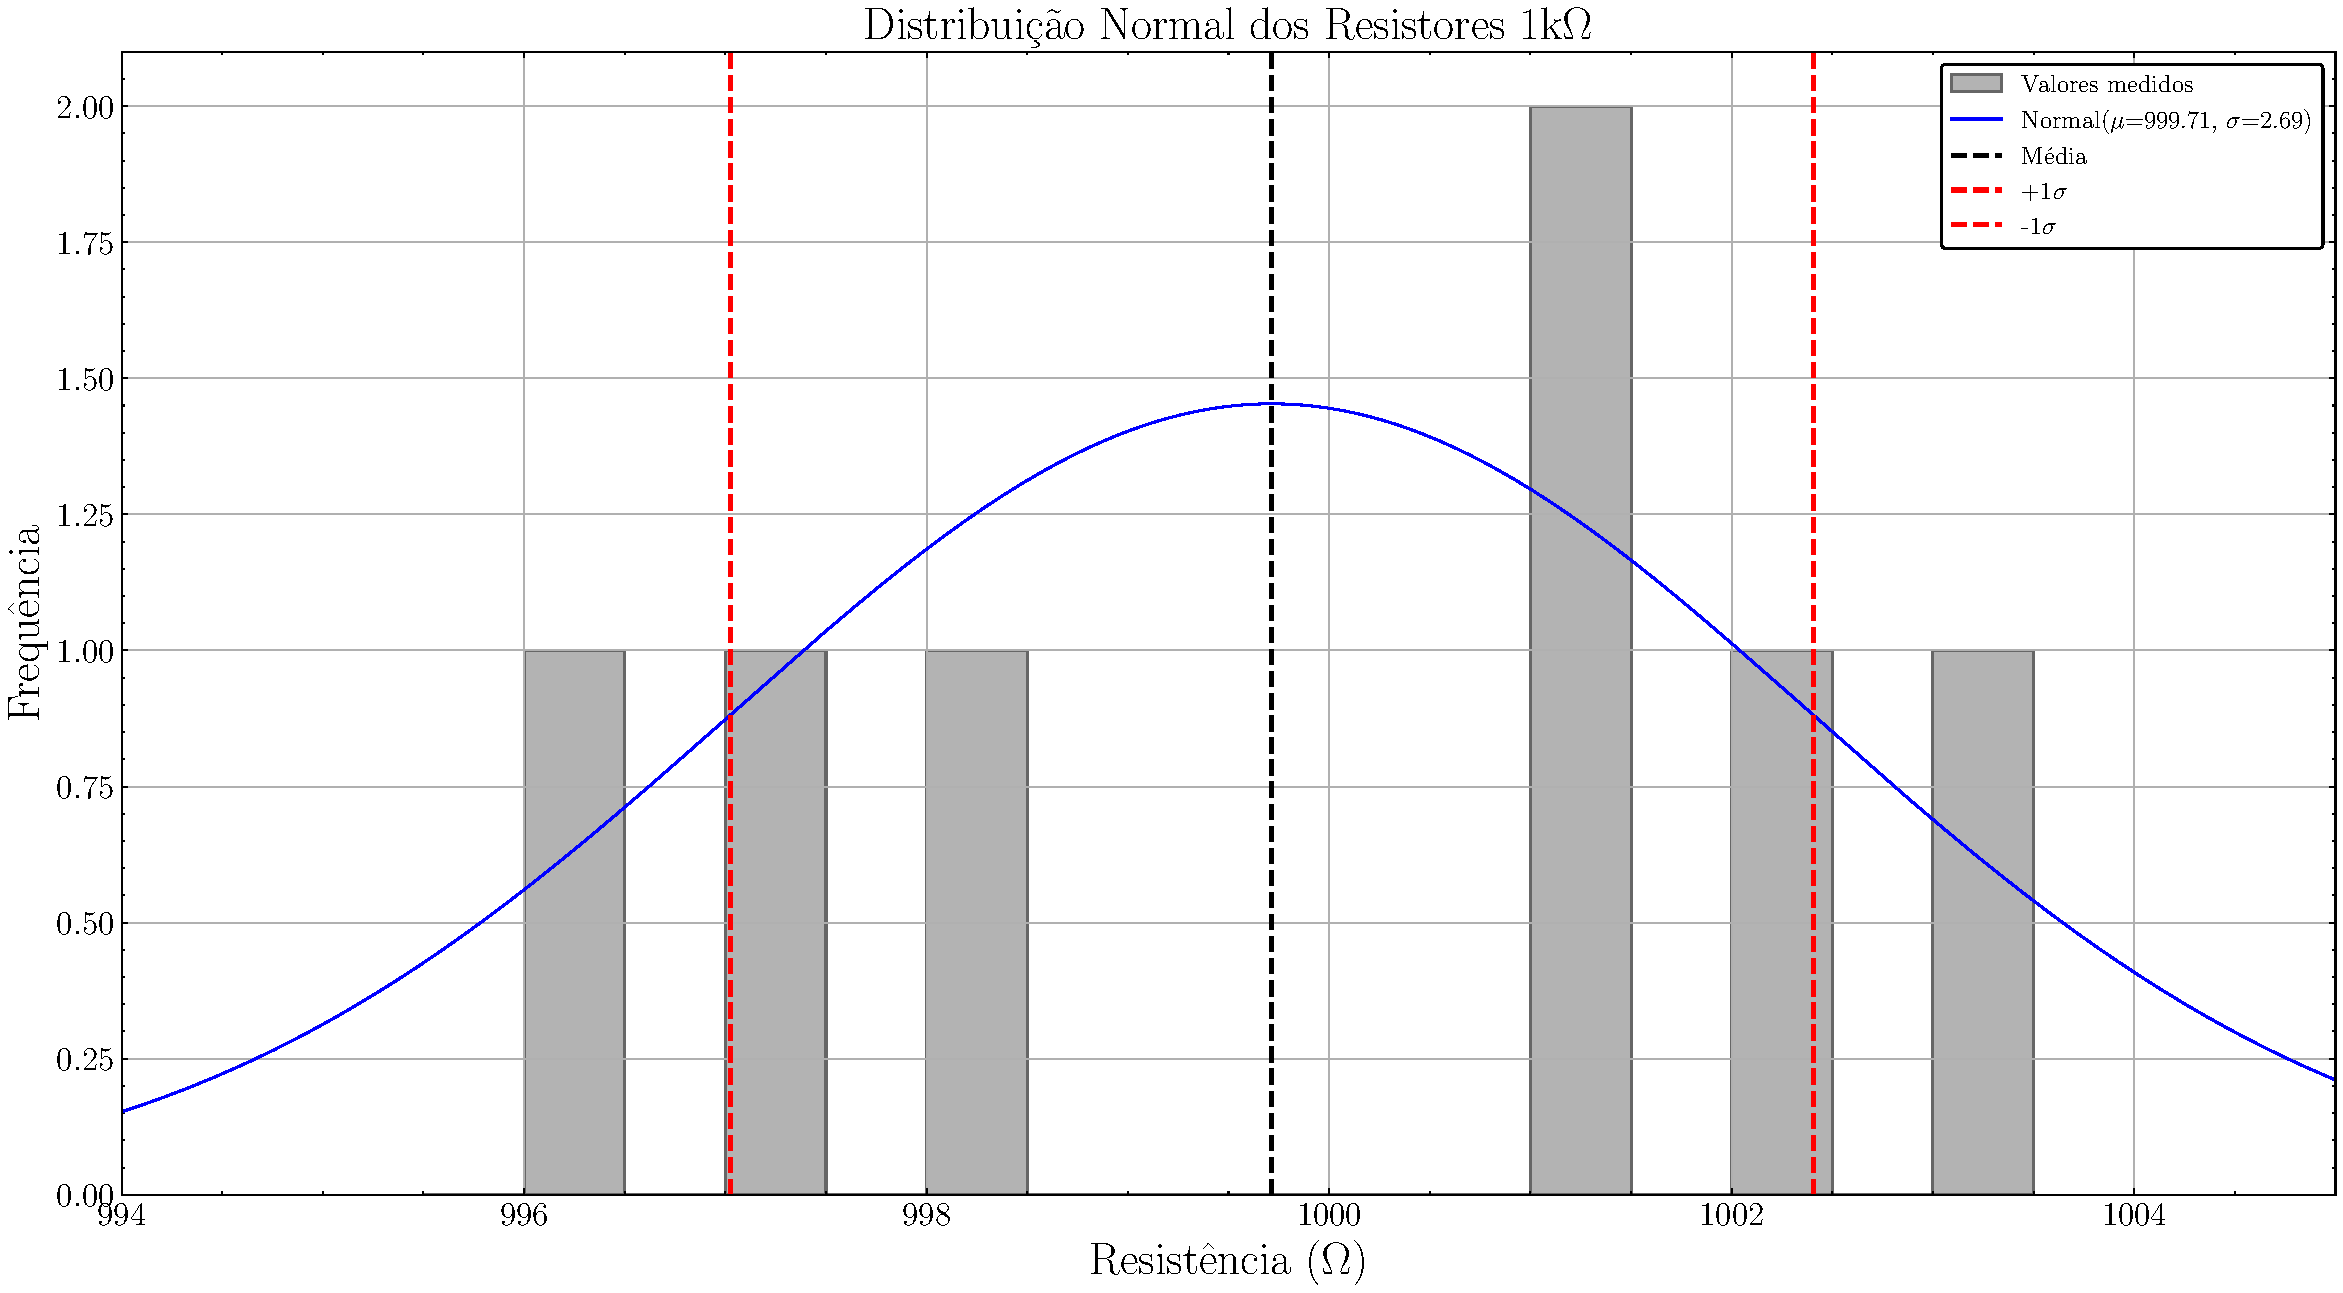
\includegraphics[width=0.8\linewidth]{figures/plot_hist_1k.pdf}
% \end{figure}

% \subsection{Associação de resistores (série, paralelo e mista)}

% O erro absoluto na associação em série é: % [COMENTARIO PROFESSOR] qual a justificativa par o uso?

% \begin{equation}
%     \sigma_{n_{eq}} = \sum_{i=1}^{n} \sigma_{n_i},
% \end{equation}
% \noindent
% Onde $\sigma_{n_{eq}}$: é a incerteza total $\sigma_{n_i}$: são as incertezas individuais de cada resistor.

% A propagação de erro para paralelo:

% \begin{equation}
%     \sigma_{n_{eq}} = R_{eq}^2 \sqrt{\sum_{i=1}^{n} \left(\frac{\sigma_{n_i}}{R_i^2}\right)^2},
% \end{equation}

% Onde $\sigma_{n_{eq}}$: é a incerteza total da associação em paralelo.
% - $\sigma_{n_i}$: são as incertezas individuais de cada resistor.
% - $R_{eq}$: é a resistência equivalente.



% \begin{align*}
%     \begin{split}
%         R_{eq} & = 1k\Omega + \left(1M\Omega || 1k\Omega\right) + \left(1M\Omega || 1M\Omega\right) \\
%                & + \left(1k\Omega || 1k\Omega\right) + 1M\Omega                                     % [COMENTARIO PROFESSOR] definir o significado do  operador de paralelo ||
%     \end{split}
% \end{align*}

% \noindent
% Podemos calcular a resistência equivalente das etapas do circuito misto, como mostrado abaixo

% \begin{figure}[htbp]
%     \centering
%     \caption{Cálculo das resistências do circuito misto}
%     \label{fig:plot_assoc_mista}
%     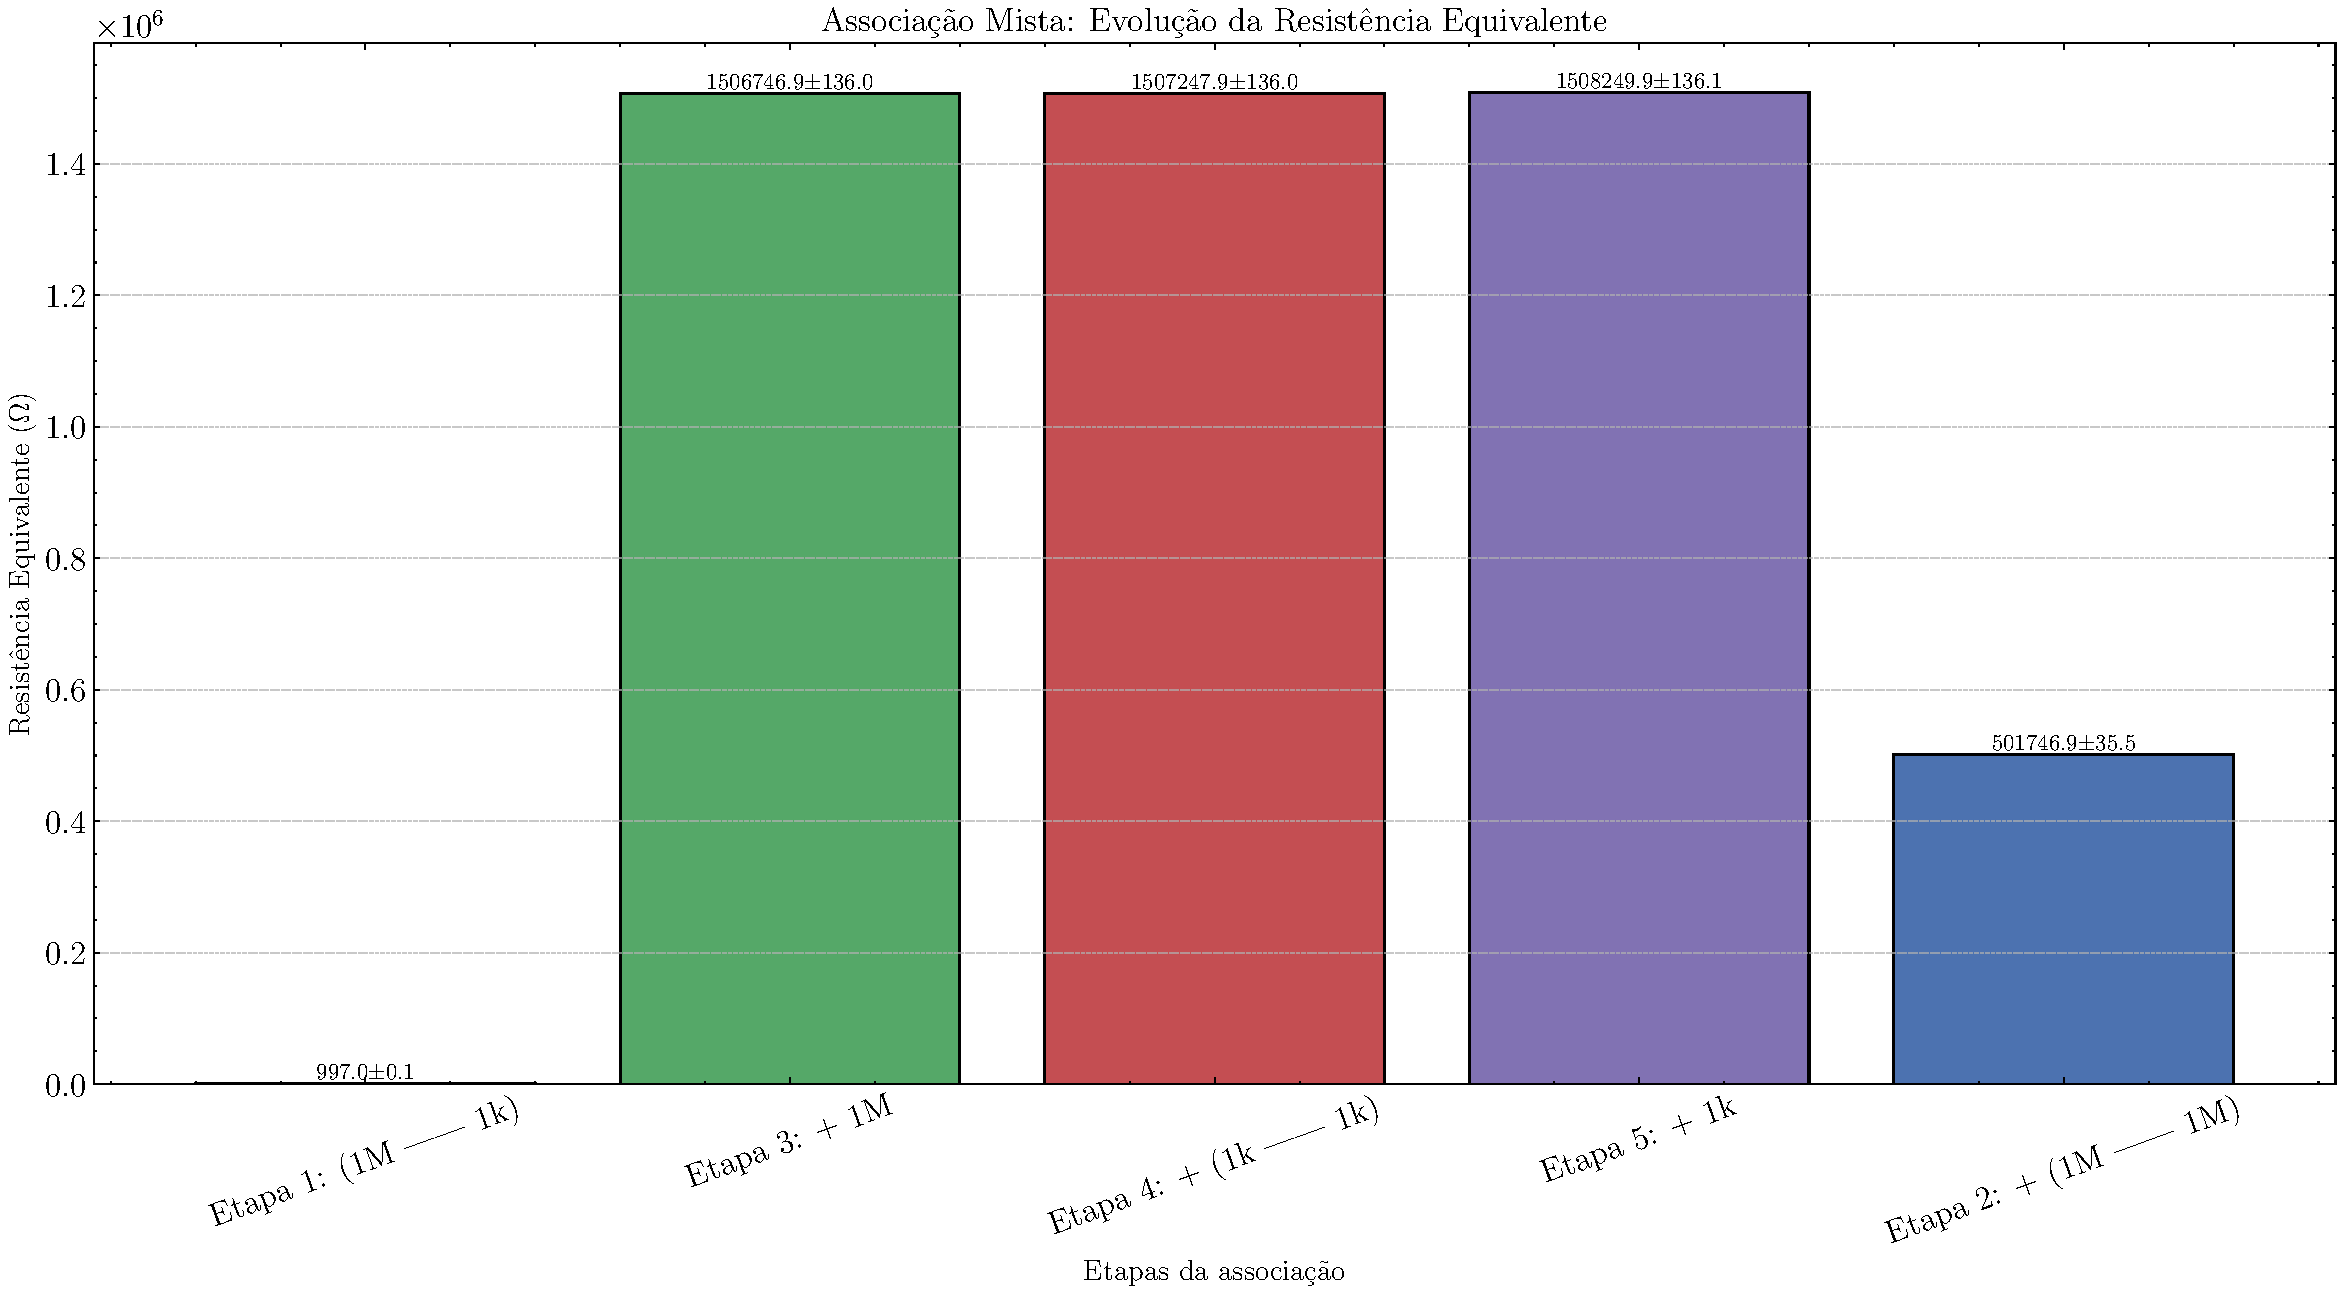
\includegraphics[width=0.8\linewidth]{figures/plot_assoc_mista.pdf}
% \end{figure}

\section{Efeito Joule}

\subsection{Aquecimento de água}

O efeito Joule refere-se à conversão da energia elétrica em energia térmica pela passagem de corrente elétrica por um condutor. Esse fenômeno está presente em aplicações como aquecedores elétricos, fusíveis, lâmpadas incandescentes e diversos processos industriais.

Neste experimento, analisou-se o aquecimento de uma amostra de água por meio da dissipação de potência elétrica em um resistor submerso. O objetivo foi verificar como a energia fornecida ao sistema contribui para o aumento da temperatura da água, considerando também as perdas térmicas para o ambiente.

A modelagem do aquecimento considerou um balanço entre a energia fornecida pela corrente elétrica e a energia dissipada para o ambiente. A equação diferencial utilizada é baseada na lei de conservação de energia térmica, com uma perda proporcional à diferença de temperatura entre a água e o ambiente, conforme descrito pela lei de resfriamento de Newton:

\begin{equation}
    \frac{dT}{dt} = \frac{P}{mc} - k (T - T_{\text{amb}})
\end{equation}

Essa equação foi adaptada de modelos clássicos de transferência de calor, como apresentado em livros-texto de física e engenharia térmica \cite{hallidayresnickwalker2023}.

\noindent
Onde \(T\) é a temperatura da água (em °C ou K), \(P\) representa a potência dissipada pelo resistor (em W), \(m\) é a massa da água (em kg), \(c\) corresponde ao calor específico da água (em J/kg·K), \(k\) é o coeficiente de troca térmica com o ambiente (em s\(^{-1}\)) e \(T_{\text{amb}}\) indica a temperatura ambiente (em °C ou K).


A equação descreve o aquecimento da água, e não o resfriamento, apesar de incorporar a taxa de perda térmica. O termo $-k(T - T_{\text{amb}})$ representa essa dissipação para o meio externo.

Para simular o comportamento do sistema ao longo do tempo, utilizou-se uma versão discretizada da equação diferencial:

\begin{equation}
    T_{i+1} = T_i + \left(\frac{P}{mc} - k (T_i - T_{\text{amb}})\right) \Delta t
\end{equation}

\noindent
Onde $T_i$ representa a temperatura no instante $i$, e $\Delta t$ representa o passo de tempo da simulação (em segundos).

\subsubsection*{Configuração experimental}

A potência $P$ foi calculada com base na tensão e corrente medidas no resistor de aquecimento. A massa da água utilizada foi de aproximadamente 500 g (0,5 kg), com calor específico $c \approx 4186\, \text{J/kg·K}$. O coeficiente $k$ foi estimado com base na inclinação da curva de resfriamento obtida experimentalmente após o desligamento da fonte de calor.

O gráfico da Figura~\ref{fig:plot_temperatura} apresenta a curva teórica de aquecimento prevista pelo modelo, juntamente com os dados experimentais. A divergência entre os dois pode ser atribuída a fatores como perdas não modeladas, imprecisão na estimativa de $k$, variações ambientais ou limitação na resposta térmica do sensor.

\begin{figure}[htbp]
    \centering
    \caption{Curva de aquecimento da água por efeito Joule}
    \label{fig:plot_temperatura}
    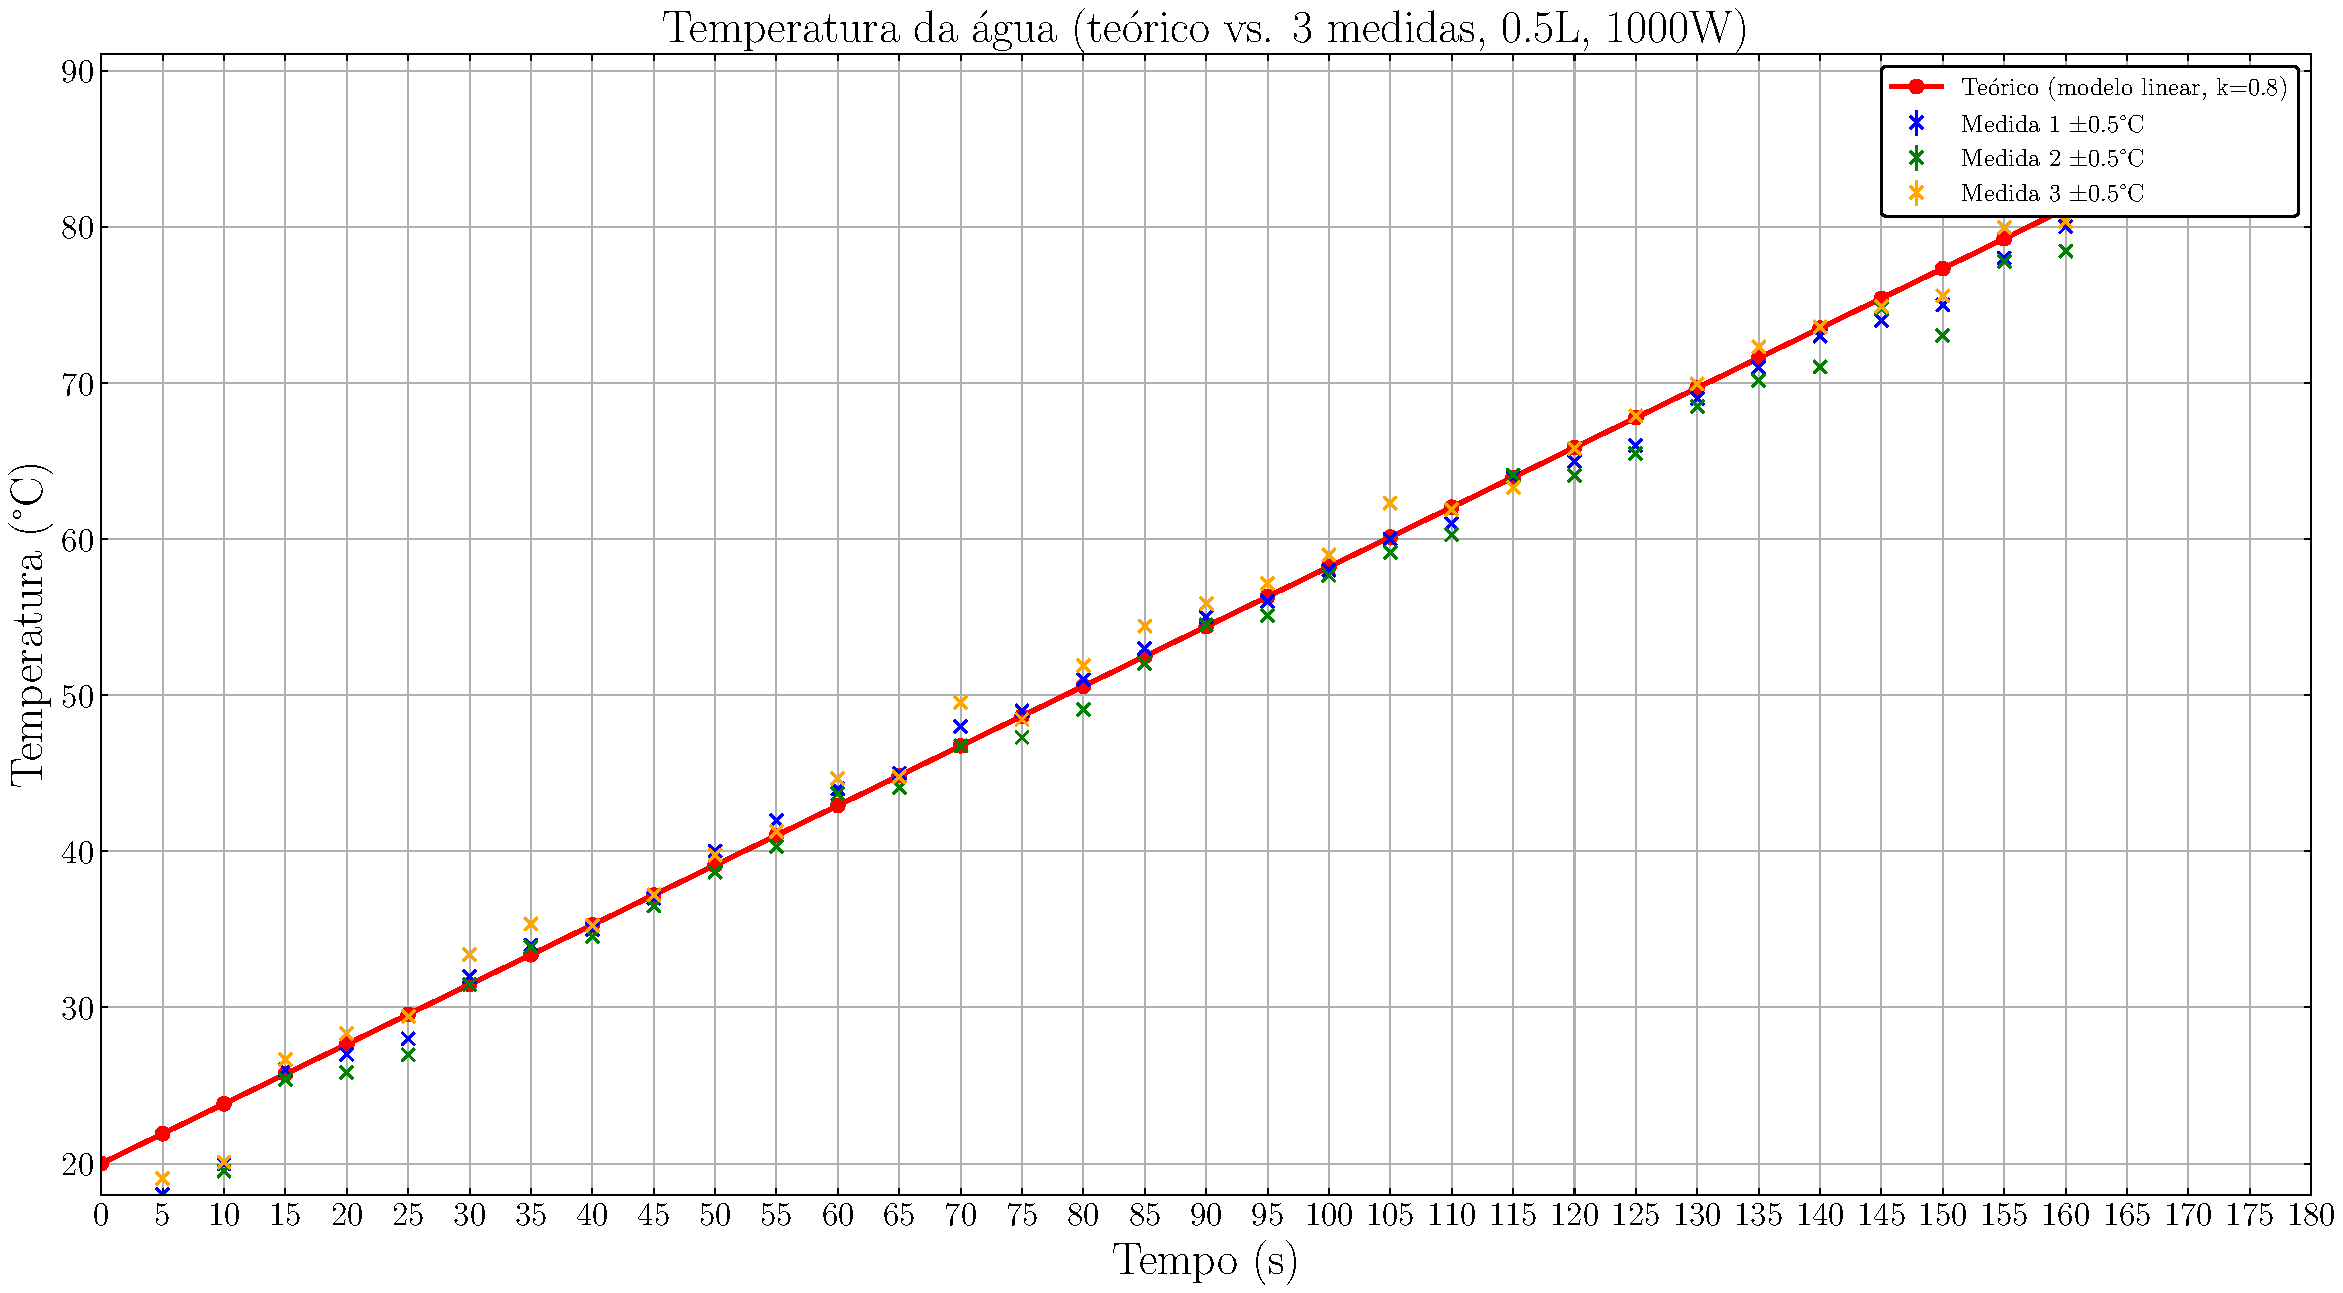
\includegraphics[width=0.8\linewidth]{figures/plot_temperatura.pdf}
\end{figure}

Compreender o efeito Joule é fundamental para o dimensionamento térmico de sistemas elétricos, tanto do ponto de vista de segurança (evitando sobreaquecimentos) quanto de eficiência energética.

% \section{Efeito Joule}

% \subsection{Aquecimento de água}

% O efeito Joule consiste na transformação da energia elétrica em energia térmica devido à passagem de corrente por um condutor ou resistor. Esse fenômeno é fundamental em aplicações como aquecedores elétricos, fusíveis, lâmpadas incandescentes e em muitos processos industriais.

% No contexto deste experimento, investigamos o aquecimento de uma amostra de água quando submetida à dissipação de potência elétrica em um resistor submerso. O objetivo é analisar como a energia fornecida ao sistema é convertida em aumento de temperatura, levando em conta também as perdas térmicas para o ambiente.

% A modelagem matemática do aquecimento é baseada na seguinte equação diferencial, que incorpora tanto o fornecimento de energia elétrica quanto a perda de calor para o ambiente (lei de Newton do resfriamento) % [COMENTARIO PROFESSOR] é resfriamento ou aquecimento?

% \begin{equation}
%     \frac{dT}{dt} = \frac{P}{mc} - k (T - T_"amb") % [COMENTARIO PROFESSOR] referenciar da onde essa equação veio
% \end{equation}

% \noindent
% Onde

% \begin{itemize}
%     \item$T$: temperatura da água (em °C ou K)
%     \item $P$: potência dissipada pelo resistor (em W)
%     \item $m$: massa da água (em kg)
%     \item $c$: calor específico da água (em J/kg·K)
%     \item $k$: coeficiente de resfriamento para o ambiente (em $s^{-1}$)
%     \item $T_"amb"$: temperatura ambiente (em °C ou K)
% \end{itemize}

% A solução numérica foi implementada de forma discreta, atualizando a temperatura a cada intervalo de tempo $d_t$:

% \begin{equation}
%     T_{i+1} = T_i + \left(\frac{P}{mc} - k (T_i - T_"amb")\right) d_t
% \end{equation}

% Onde $T_i$: temperatura no instante $i$, $d_t$: passo de tempo da simulação, medido em segundos.

% Configuração experimental:
% \begin{itemize}
%     \item A potência $P$ foi calculada a partir da tensão e corrente aplicadas ao resistor.
%     \item A massa $m$ da água e o calor específico $c$ são conhecidos.
%     \item O coeficiente $k$ foi estimado a partir da taxa de resfriamento observada experimentalmente.
% \end{itemize}

% O gráfico a seguir apresenta a evolução da temperatura da água ao longo do tempo, mostrando tanto a curva teórica prevista pelo modelo quanto dados experimentais simulados. A diferença entre as curvas pode ser atribuída a fatores como perdas adicionais, imprecisão na medição de $k$ ou variações ambientais.

% \begin{figure}[htbp]
%     \centering
%     \caption{Curva de aquecimento da água por efeito Joule}
%     \label{fig:plot_temperatura}
%     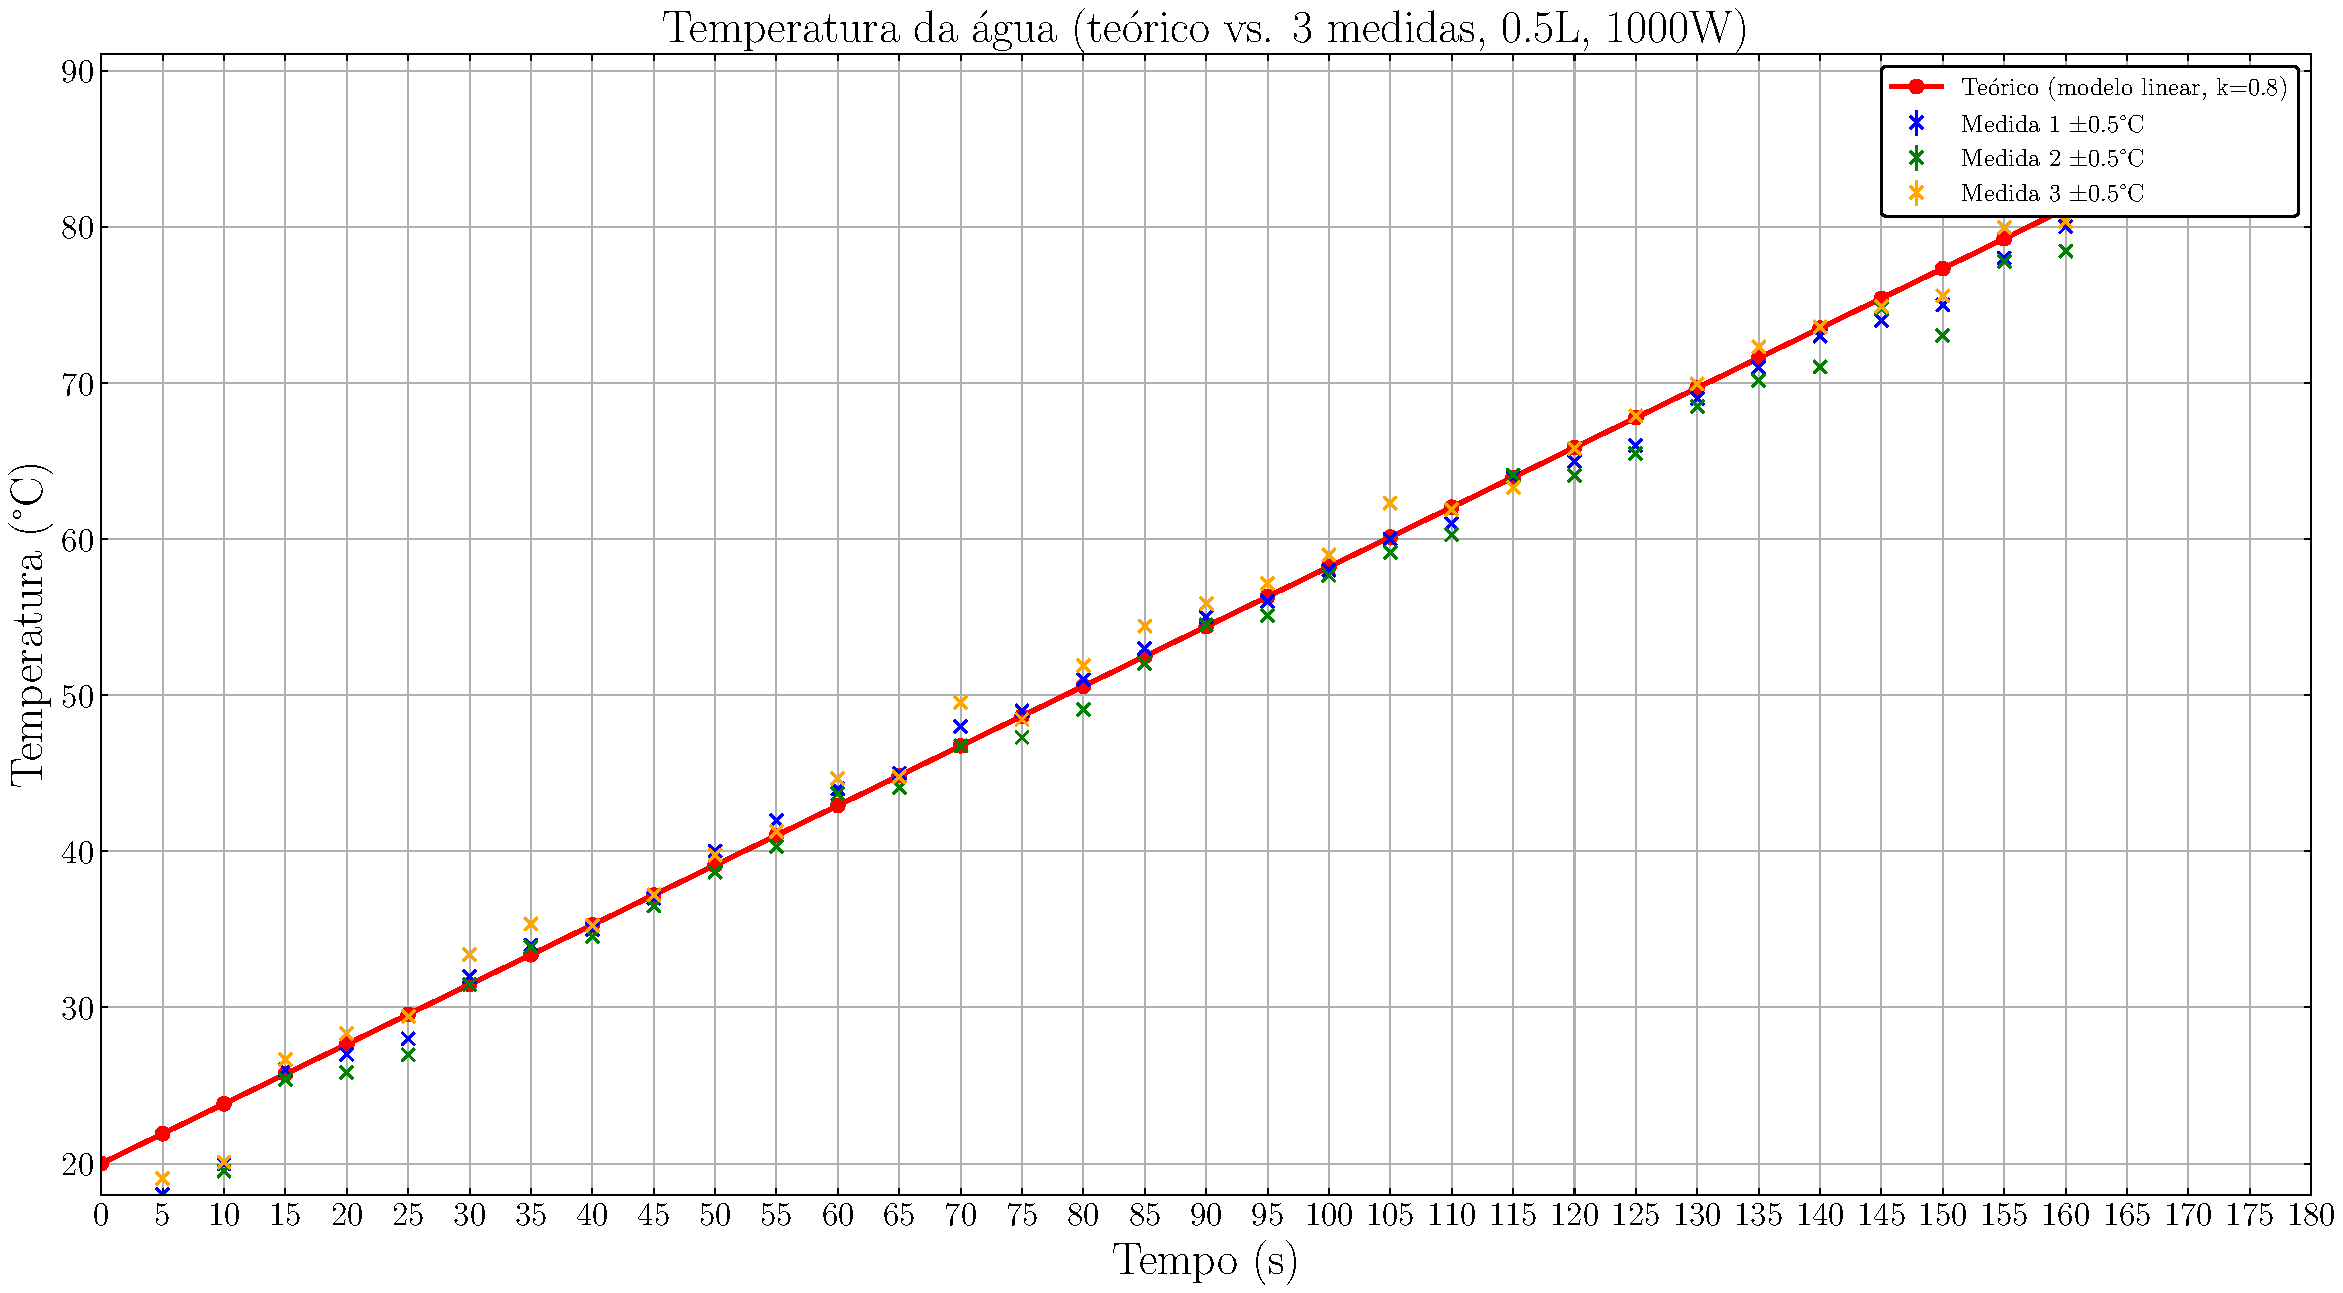
\includegraphics[width=0.8\linewidth]{figures/plot_temperatura.pdf}
% \end{figure}

% O estudo do efeito Joule é essencial para o dimensionamento seguro de dispositivos elétricos, evitando sobreaquecimento e otimizando a eficiência energética de sistemas de aquecimento.

\section{Conclusão} % [COMENTARIO PROFESSOR] está muito pedagógico e pouco científico, quero ver a análise dos resistores e o efeito Joule

O presente estudo forneceu uma análise detalhada das associações de resistores em configurações série, paralelo e mista, evidenciando a variação da resistência equivalente e a influência das tolerâncias dos componentes. As medições realizadas, acompanhadas de análise estatística rigorosa, permitiram quantificar as incertezas experimentais, destacando que a consideração dos erros de medição é fundamental para uma avaliação precisa e confiável dos resultados. Observou-se que, embora as resistências nominais indiquem valores teóricos, a dispersão dos valores reais e as incertezas associadas impactam significativamente no desempenho dos circuitos montados.

No que diz respeito ao efeito Joule, a experimentação demonstrou claramente a conversão de energia elétrica em energia térmica, com a evolução da temperatura da água refletindo a dissipação de potência pelo resistor. A modelagem matemática, baseada em um balanço energético incluindo perdas térmicas por convecção, mostrou-se eficaz na previsão do comportamento térmico do sistema, embora divergências entre modelo e dados experimentais evidenciem a complexidade dos processos de transferência de calor reais. Esses resultados ressaltam a importância da inclusão de fatores ambientais e da caracterização precisa dos coeficientes de troca térmica para o dimensionamento seguro e eficiente de dispositivos que operam sob regimes de dissipação térmica.

Em síntese, este trabalho reforça a necessidade do rigor experimental e da análise crítica na engenharia elétrica, demonstrando que a precisão nas medições e a adequação dos modelos físicos são essenciais para a otimização e segurança dos sistemas eletrônicos e térmicos. A experiência adquirida contribui para o aprimoramento das competências técnicas dos profissionais, fundamentais para o desenvolvimento de soluções confiáveis e eficientes no campo da engenharia.


% O experimento permitiu compreender, na prática, os princípios fundamentais das associações de resistores em série, paralelo e mista, bem como a influência dessas configurações na resistência equivalente de um circuito. As medições e análises estatísticas mostraram a importância de considerar as tolerâncias e incertezas dos componentes, reforçando a necessidade do cálculo de erros experimentais para uma avaliação precisa dos resultados.

% A investigação do efeito Joule demonstrou como a energia elétrica é convertida em calor, evidenciando o papel dos resistores como elementos dissipadores. A modelagem matemática e a comparação com dados experimentais destacaram a relevância de fatores como perdas térmicas e transferência de calor para o ambiente, aspectos essenciais para o dimensionamento seguro de dispositivos elétricos.

% Além de consolidar conceitos teóricos, o experimento proporcionou experiência com instrumentos de medição e análise de dados, habilidades essenciais para a formação em Engenharia. O estudo reforça a importância do rigor experimental e da análise crítica dos resultados, fundamentais para o desenvolvimento de soluções eficientes e seguras em projetos eletrônicos e sistemas de energia.

\bibliographystyle{IEEEtran}
\bibliography{references}

\end{document}
